\batchmode
\documentclass[twoside]{book}

% Packages required by doxygen
\usepackage{fixltx2e}
\usepackage{calc}
\usepackage{doxygen}
\usepackage[export]{adjustbox} % also loads graphicx
\usepackage{graphicx}
\usepackage[utf8]{inputenc}
\usepackage{makeidx}
\usepackage{multicol}
\usepackage{multirow}
\PassOptionsToPackage{warn}{textcomp}
\usepackage{textcomp}
\usepackage[nointegrals]{wasysym}
\usepackage[table]{xcolor}

% Font selection
\usepackage[T1]{fontenc}
\usepackage[scaled=.90]{helvet}
\usepackage{courier}
\usepackage{amssymb}
\usepackage{sectsty}
\renewcommand{\familydefault}{\sfdefault}
\allsectionsfont{%
  \fontseries{bc}\selectfont%
  \color{darkgray}%
}
\renewcommand{\DoxyLabelFont}{%
  \fontseries{bc}\selectfont%
  \color{darkgray}%
}
\newcommand{\+}{\discretionary{\mbox{\scriptsize$\hookleftarrow$}}{}{}}

% Page & text layout
\usepackage{geometry}
\geometry{%
  a4paper,%
  top=2.5cm,%
  bottom=2.5cm,%
  left=2.5cm,%
  right=2.5cm%
}
\tolerance=750
\hfuzz=15pt
\hbadness=750
\setlength{\emergencystretch}{15pt}
\setlength{\parindent}{0cm}
\setlength{\parskip}{3ex plus 2ex minus 2ex}
\makeatletter
\renewcommand{\paragraph}{%
  \@startsection{paragraph}{4}{0ex}{-1.0ex}{1.0ex}{%
    \normalfont\normalsize\bfseries\SS@parafont%
  }%
}
\renewcommand{\subparagraph}{%
  \@startsection{subparagraph}{5}{0ex}{-1.0ex}{1.0ex}{%
    \normalfont\normalsize\bfseries\SS@subparafont%
  }%
}
\makeatother

% Headers & footers
\usepackage{fancyhdr}
\pagestyle{fancyplain}
\fancyhead[LE]{\fancyplain{}{\bfseries\thepage}}
\fancyhead[CE]{\fancyplain{}{}}
\fancyhead[RE]{\fancyplain{}{\bfseries\leftmark}}
\fancyhead[LO]{\fancyplain{}{\bfseries\rightmark}}
\fancyhead[CO]{\fancyplain{}{}}
\fancyhead[RO]{\fancyplain{}{\bfseries\thepage}}
\fancyfoot[LE]{\fancyplain{}{}}
\fancyfoot[CE]{\fancyplain{}{}}
\fancyfoot[RE]{\fancyplain{}{\bfseries\scriptsize Generated by Doxygen }}
\fancyfoot[LO]{\fancyplain{}{\bfseries\scriptsize Generated by Doxygen }}
\fancyfoot[CO]{\fancyplain{}{}}
\fancyfoot[RO]{\fancyplain{}{}}
\renewcommand{\footrulewidth}{0.4pt}
\renewcommand{\chaptermark}[1]{%
  \markboth{#1}{}%
}
\renewcommand{\sectionmark}[1]{%
  \markright{\thesection\ #1}%
}

% Indices & bibliography
\usepackage{natbib}
\usepackage[titles]{tocloft}
\setcounter{tocdepth}{3}
\setcounter{secnumdepth}{5}
\makeindex

% Hyperlinks (required, but should be loaded last)
\usepackage{ifpdf}
\ifpdf
  \usepackage[pdftex,pagebackref=true]{hyperref}
\else
  \usepackage[ps2pdf,pagebackref=true]{hyperref}
\fi
\hypersetup{%
  colorlinks=true,%
  linkcolor=blue,%
  citecolor=blue,%
  unicode%
}

% Custom commands
\newcommand{\clearemptydoublepage}{%
  \newpage{\pagestyle{empty}\cleardoublepage}%
}

\usepackage{caption}
\captionsetup{labelsep=space,justification=centering,font={bf},singlelinecheck=off,skip=4pt,position=top}

%===== C O N T E N T S =====

\begin{document}

% Titlepage & ToC
\hypersetup{pageanchor=false,
             bookmarksnumbered=true,
             pdfencoding=unicode
            }
\pagenumbering{alph}
\pagenumbering{arabic}
\hypersetup{pageanchor=true}

%--- Begin generated contents ---
\chapter{Example problem\+: The spatially-\/adaptive solution of the azimuthally Fourier-\/decomposed 3D Helmholtz equation}
\label{index}\hypertarget{index}{}\hypertarget{index_q}{}\section{A few quick questions...}\label{index_q}
Since {\ttfamily oomph-\/lib} is developed as open-\/source software, any evidence that the code is being downloaded and used is very helpful for us as it helps to justify our continued work on this project.

We would therefore be extremely grateful if you could provide the information requested in the form below. Pressing the \char`\"{}submit\char`\"{} button will get you to the actual download page.

{\bfseries Note\+:} 
\begin{DoxyItemize}
\item All information will be treated as confidential. 
\item If you provide your email address and check the appropriate box we will add you to our mailing list to inform you of upgrades and bug fixes to the code. Rest assured that the mailing list is {\bfseries very low volume} -- we have better things to do than to bombard you with email. 
\item If you still feel reluctant to provide any of the information requested, feel free to enter some dummy input. The form will check that {\bfseries some} information has been entered but entering your name as \char`\"{}\+Joe Cool\char`\"{} is perfectly acceptable -- this is to discourage people from not providing the information simply because they are too lazy to type... 
\end{DoxyItemize}



 







 

 \hypertarget{index_pdf}{}\section{P\+D\+F file}\label{index_pdf}
A \href{../latex/refman.pdf}{\tt pdf version} of this document is available. \end{document}

\chapter{Namespace Index}
\section{Namespace List}
Here is a list of all namespaces with brief descriptions\+:\begin{DoxyCompactList}
\item\contentsline{section}{\hyperlink{namespaceGlobal__Physical__Variables}{Global\+\_\+\+Physical\+\_\+\+Variables} \\*Global variables that represent physical properties }{\pageref{namespaceGlobal__Physical__Variables}}{}
\item\contentsline{section}{\hyperlink{namespaceoomph}{oomph} }{\pageref{namespaceoomph}}{}
\item\contentsline{section}{\hyperlink{namespacePhysical__Variables}{Physical\+\_\+\+Variables} \\*Namespace for the solution of 2D linear shell equation }{\pageref{namespacePhysical__Variables}}{}
\end{DoxyCompactList}

\chapter{Hierarchical Index}
\section{Class Hierarchy}
This inheritance list is sorted roughly, but not completely, alphabetically\+:\begin{DoxyCompactList}
\item Problem\begin{DoxyCompactList}
\item \contentsline{section}{Unstructured\+Solid\+Problem$<$ E\+L\+E\+M\+E\+NT $>$}{\pageref{classUnstructuredSolidProblem}}{}
\end{DoxyCompactList}
\end{DoxyCompactList}

\chapter{Class Index}
\section{Class List}
Here are the classes, structs, unions and interfaces with brief descriptions\+:\begin{DoxyCompactList}
\item\contentsline{section}{\hyperlink{classPMLProblem}{P\+M\+L\+Problem$<$ E\+L\+E\+M\+E\+N\+T $>$} }{\pageref{classPMLProblem}}{}
\item\contentsline{section}{\hyperlink{classGlobalParameters_1_1TestPMLMapping}{Global\+Parameters\+::\+Test\+P\+M\+L\+Mapping} }{\pageref{classGlobalParameters_1_1TestPMLMapping}}{}
\end{DoxyCompactList}

\chapter{File Index}
\section{File List}
Here is a list of all files with brief descriptions\+:\begin{DoxyCompactList}
\item\contentsline{section}{\hyperlink{jeffery__orbit_8cc}{jeffery\+\_\+orbit.\+cc} }{\pageref{jeffery__orbit_8cc}}{}
\item\contentsline{section}{\hyperlink{jeffery__orbit_8txt__doxygenified_8h}{jeffery\+\_\+orbit.\+txt\+\_\+doxygenified.\+h} }{\pageref{jeffery__orbit_8txt__doxygenified_8h}}{}
\item\contentsline{section}{\hyperlink{my__taylor__hood__elements_8h}{my\+\_\+taylor\+\_\+hood\+\_\+elements.\+h} }{\pageref{my__taylor__hood__elements_8h}}{}
\end{DoxyCompactList}

\chapter{Namespace Documentation}
\hypertarget{namespacePlanarWave}{}\section{Planar\+Wave Namespace Reference}
\label{namespacePlanarWave}\index{Planar\+Wave@{Planar\+Wave}}
\subsection*{Functions}
\begin{DoxyCompactItemize}
\item 
std\+::complex$<$ double $>$ \hyperlink{namespacePlanarWave_a541691caf71477c8c389062797c0fdab}{I} (0.\+0, 1.\+0)
\begin{DoxyCompactList}\small\item\em Imaginary unit. \end{DoxyCompactList}\item 
void \hyperlink{namespacePlanarWave_a00f252bcf0181187c656a58ce36b07b5}{get\+\_\+exact\+\_\+u} (const Vector$<$ double $>$ \&x, Vector$<$ double $>$ \&u)
\begin{DoxyCompactList}\small\item\em Exact solution as a Vector of size 2, containing real and imag parts. \end{DoxyCompactList}\item 
void \hyperlink{namespacePlanarWave_afe1e9812d1b1dc40a89f7a1f18d1165f}{plot} ()
\begin{DoxyCompactList}\small\item\em Plot. \end{DoxyCompactList}\end{DoxyCompactItemize}
\subsection*{Variables}
\begin{DoxyCompactItemize}
\item 
unsigned \hyperlink{namespacePlanarWave_a56abdb2474ccaffd88346ee3607d8672}{N\+\_\+terms} =100
\begin{DoxyCompactList}\small\item\em Number of terms in series. \end{DoxyCompactList}\item 
double \hyperlink{namespacePlanarWave_a1d51c00058fbc80aa9d255fffd92abac}{K} =3.\+0$\ast$Mathematical\+Constants\+::\+Pi
\begin{DoxyCompactList}\small\item\em Wave number. \end{DoxyCompactList}\end{DoxyCompactItemize}


\subsection{Detailed Description}
Namespace to test representation of planar wave in spherical polars 

\subsection{Function Documentation}
\mbox{\Hypertarget{namespacePlanarWave_a00f252bcf0181187c656a58ce36b07b5}\label{namespacePlanarWave_a00f252bcf0181187c656a58ce36b07b5}} 
\index{Planar\+Wave@{Planar\+Wave}!get\+\_\+exact\+\_\+u@{get\+\_\+exact\+\_\+u}}
\index{get\+\_\+exact\+\_\+u@{get\+\_\+exact\+\_\+u}!Planar\+Wave@{Planar\+Wave}}
\subsubsection{\texorpdfstring{get\+\_\+exact\+\_\+u()}{get\_exact\_u()}}
{\footnotesize\ttfamily void Planar\+Wave\+::get\+\_\+exact\+\_\+u (\begin{DoxyParamCaption}\item[{const Vector$<$ double $>$ \&}]{x,  }\item[{Vector$<$ double $>$ \&}]{u }\end{DoxyParamCaption})}



Exact solution as a Vector of size 2, containing real and imag parts. 



Definition at line 125 of file sphere\+\_\+scattering.\+cc.



References Problem\+Parameters\+::\+I(), and Problem\+Parameters\+::\+N\+\_\+terms.

\mbox{\Hypertarget{namespacePlanarWave_a541691caf71477c8c389062797c0fdab}\label{namespacePlanarWave_a541691caf71477c8c389062797c0fdab}} 
\index{Planar\+Wave@{Planar\+Wave}!I@{I}}
\index{I@{I}!Planar\+Wave@{Planar\+Wave}}
\subsubsection{\texorpdfstring{I()}{I()}}
{\footnotesize\ttfamily std\+::complex$<$ double $>$ Planar\+Wave\+::I (\begin{DoxyParamCaption}\item[{0.}]{0,  }\item[{1.}]{0 }\end{DoxyParamCaption})}



Imaginary unit. 

\mbox{\Hypertarget{namespacePlanarWave_afe1e9812d1b1dc40a89f7a1f18d1165f}\label{namespacePlanarWave_afe1e9812d1b1dc40a89f7a1f18d1165f}} 
\index{Planar\+Wave@{Planar\+Wave}!plot@{plot}}
\index{plot@{plot}!Planar\+Wave@{Planar\+Wave}}
\subsubsection{\texorpdfstring{plot()}{plot()}}
{\footnotesize\ttfamily void Planar\+Wave\+::plot (\begin{DoxyParamCaption}{ }\end{DoxyParamCaption})}



Plot. 



Definition at line 184 of file sphere\+\_\+scattering.\+cc.



References Problem\+Parameters\+::get\+\_\+exact\+\_\+u(), and Problem\+Parameters\+::\+I().



\subsection{Variable Documentation}
\mbox{\Hypertarget{namespacePlanarWave_a1d51c00058fbc80aa9d255fffd92abac}\label{namespacePlanarWave_a1d51c00058fbc80aa9d255fffd92abac}} 
\index{Planar\+Wave@{Planar\+Wave}!K@{K}}
\index{K@{K}!Planar\+Wave@{Planar\+Wave}}
\subsubsection{\texorpdfstring{K}{K}}
{\footnotesize\ttfamily double Planar\+Wave\+::K =3.\+0$\ast$Mathematical\+Constants\+::\+Pi}



Wave number. 



Definition at line 119 of file sphere\+\_\+scattering.\+cc.

\mbox{\Hypertarget{namespacePlanarWave_a56abdb2474ccaffd88346ee3607d8672}\label{namespacePlanarWave_a56abdb2474ccaffd88346ee3607d8672}} 
\index{Planar\+Wave@{Planar\+Wave}!N\+\_\+terms@{N\+\_\+terms}}
\index{N\+\_\+terms@{N\+\_\+terms}!Planar\+Wave@{Planar\+Wave}}
\subsubsection{\texorpdfstring{N\+\_\+terms}{N\_terms}}
{\footnotesize\ttfamily unsigned Planar\+Wave\+::\+N\+\_\+terms =100}



Number of terms in series. 



Definition at line 116 of file sphere\+\_\+scattering.\+cc.


\hypertarget{namespaceProblemParameters}{}\section{Problem\+Parameters Namespace Reference}
\label{namespaceProblemParameters}\index{Problem\+Parameters@{Problem\+Parameters}}


Namespace for the Fourier decomposed Helmholtz problem parameters.  


\subsection*{Functions}
\begin{DoxyCompactItemize}
\item 
Vector$<$ double $>$ \hyperlink{namespaceProblemParameters_acb1788444ef78fe2adec824504f24246}{Coeff} (\hyperlink{namespaceProblemParameters_a6361f0f1c4a120e62d28db64baa84b40}{N\+\_\+terms}, 1.\+0)
\begin{DoxyCompactList}\small\item\em Coefficients in the exact solution. \end{DoxyCompactList}\item 
std\+::complex$<$ double $>$ \hyperlink{namespaceProblemParameters_acfe6a3fe73272672d596ebe2afd0092e}{I} (0.\+0, 1.\+0)
\begin{DoxyCompactList}\small\item\em Imaginary unit. \end{DoxyCompactList}\item 
void \hyperlink{namespaceProblemParameters_af750b29069b29bd38b5220ecf534e7f7}{get\+\_\+exact\+\_\+u} (const Vector$<$ double $>$ \&x, Vector$<$ double $>$ \&u)
\begin{DoxyCompactList}\small\item\em Exact solution as a Vector of size 2, containing real and imag parts. \end{DoxyCompactList}\item 
void \hyperlink{namespaceProblemParameters_aa544d1f3e384d3283f7113512931ea8f}{exact\+\_\+minus\+\_\+dudr} (const Vector$<$ double $>$ \&x, std\+::complex$<$ double $>$ \&flux)
\begin{DoxyCompactList}\small\item\em Get -\/du/dr (spherical r) for exact solution. Equal to prescribed flux on inner boundary. \end{DoxyCompactList}\end{DoxyCompactItemize}
\subsection*{Variables}
\begin{DoxyCompactItemize}
\item 
double \hyperlink{namespaceProblemParameters_aa5362de1af9e257fde4317c367158a93}{K\+\_\+squared} =10.\+0
\begin{DoxyCompactList}\small\item\em Square of the wavenumber. \end{DoxyCompactList}\item 
int \hyperlink{namespaceProblemParameters_aaa674958a1ca6ee0b99de3377288c93f}{N\+\_\+fourier} =3
\begin{DoxyCompactList}\small\item\em Fourier wave number. \end{DoxyCompactList}\item 
unsigned \hyperlink{namespaceProblemParameters_aa529b33b7feb959e0c044447bf0f6c6f}{Nterms\+\_\+for\+\_\+\+DtN} =6
\begin{DoxyCompactList}\small\item\em Number of terms in computation of DtN boundary condition. \end{DoxyCompactList}\item 
unsigned \hyperlink{namespaceProblemParameters_a6361f0f1c4a120e62d28db64baa84b40}{N\+\_\+terms} =6
\begin{DoxyCompactList}\small\item\em Number of terms in the exact solution. \end{DoxyCompactList}\item 
unsigned \hyperlink{namespaceProblemParameters_a23b618b9e3a0d282fd91aa3f3f7b9254}{El\+\_\+multiplier} =1
\begin{DoxyCompactList}\small\item\em Multiplier for number of elements. \end{DoxyCompactList}\end{DoxyCompactItemize}


\subsection{Detailed Description}
Namespace for the Fourier decomposed Helmholtz problem parameters. 

\subsection{Function Documentation}
\mbox{\Hypertarget{namespaceProblemParameters_acb1788444ef78fe2adec824504f24246}\label{namespaceProblemParameters_acb1788444ef78fe2adec824504f24246}} 
\index{Problem\+Parameters@{Problem\+Parameters}!Coeff@{Coeff}}
\index{Coeff@{Coeff}!Problem\+Parameters@{Problem\+Parameters}}
\subsubsection{\texorpdfstring{Coeff()}{Coeff()}}
{\footnotesize\ttfamily Vector$<$ double $>$ Problem\+Parameters\+::\+Coeff (\begin{DoxyParamCaption}\item[{\hyperlink{namespaceProblemParameters_a6361f0f1c4a120e62d28db64baa84b40}{N\+\_\+terms}}]{,  }\item[{1.}]{0 }\end{DoxyParamCaption})}



Coefficients in the exact solution. 



Referenced by exact\+\_\+minus\+\_\+dudr(), and get\+\_\+exact\+\_\+u().

\mbox{\Hypertarget{namespaceProblemParameters_aa544d1f3e384d3283f7113512931ea8f}\label{namespaceProblemParameters_aa544d1f3e384d3283f7113512931ea8f}} 
\index{Problem\+Parameters@{Problem\+Parameters}!exact\+\_\+minus\+\_\+dudr@{exact\+\_\+minus\+\_\+dudr}}
\index{exact\+\_\+minus\+\_\+dudr@{exact\+\_\+minus\+\_\+dudr}!Problem\+Parameters@{Problem\+Parameters}}
\subsubsection{\texorpdfstring{exact\+\_\+minus\+\_\+dudr()}{exact\_minus\_dudr()}}
{\footnotesize\ttfamily void Problem\+Parameters\+::exact\+\_\+minus\+\_\+dudr (\begin{DoxyParamCaption}\item[{const Vector$<$ double $>$ \&}]{x,  }\item[{std\+::complex$<$ double $>$ \&}]{flux }\end{DoxyParamCaption})}



Get -\/du/dr (spherical r) for exact solution. Equal to prescribed flux on inner boundary. 



Definition at line 306 of file sphere\+\_\+scattering.\+cc.



References Coeff(), I(), and N\+\_\+terms.



Referenced by Fourier\+Decomposed\+Helmholtz\+Problem$<$ E\+L\+E\+M\+E\+N\+T $>$\+::actions\+\_\+after\+\_\+adapt(), Fourier\+Decomposed\+Helmholtz\+Problem$<$ E\+L\+E\+M\+E\+N\+T $>$\+::check\+\_\+gamma(), and Fourier\+Decomposed\+Helmholtz\+Problem$<$ E\+L\+E\+M\+E\+N\+T $>$\+::create\+\_\+flux\+\_\+elements\+\_\+on\+\_\+inner\+\_\+boundary().

\mbox{\Hypertarget{namespaceProblemParameters_af750b29069b29bd38b5220ecf534e7f7}\label{namespaceProblemParameters_af750b29069b29bd38b5220ecf534e7f7}} 
\index{Problem\+Parameters@{Problem\+Parameters}!get\+\_\+exact\+\_\+u@{get\+\_\+exact\+\_\+u}}
\index{get\+\_\+exact\+\_\+u@{get\+\_\+exact\+\_\+u}!Problem\+Parameters@{Problem\+Parameters}}
\subsubsection{\texorpdfstring{get\+\_\+exact\+\_\+u()}{get\_exact\_u()}}
{\footnotesize\ttfamily void Problem\+Parameters\+::get\+\_\+exact\+\_\+u (\begin{DoxyParamCaption}\item[{const Vector$<$ double $>$ \&}]{x,  }\item[{Vector$<$ double $>$ \&}]{u }\end{DoxyParamCaption})}



Exact solution as a Vector of size 2, containing real and imag parts. 



Definition at line 247 of file sphere\+\_\+scattering.\+cc.



References Coeff(), I(), and N\+\_\+terms.



Referenced by Fourier\+Decomposed\+Helmholtz\+Problem$<$ E\+L\+E\+M\+E\+N\+T $>$\+::actions\+\_\+after\+\_\+adapt(), Fourier\+Decomposed\+Helmholtz\+Problem$<$ E\+L\+E\+M\+E\+N\+T $>$\+::doc\+\_\+solution(), and Planar\+Wave\+::plot().

\mbox{\Hypertarget{namespaceProblemParameters_acfe6a3fe73272672d596ebe2afd0092e}\label{namespaceProblemParameters_acfe6a3fe73272672d596ebe2afd0092e}} 
\index{Problem\+Parameters@{Problem\+Parameters}!I@{I}}
\index{I@{I}!Problem\+Parameters@{Problem\+Parameters}}
\subsubsection{\texorpdfstring{I()}{I()}}
{\footnotesize\ttfamily std\+::complex$<$ double $>$ Problem\+Parameters\+::I (\begin{DoxyParamCaption}\item[{0.}]{0,  }\item[{1.}]{0 }\end{DoxyParamCaption})}



Imaginary unit. 



Referenced by exact\+\_\+minus\+\_\+dudr(), Planar\+Wave\+::get\+\_\+exact\+\_\+u(), get\+\_\+exact\+\_\+u(), and Planar\+Wave\+::plot().



\subsection{Variable Documentation}
\mbox{\Hypertarget{namespaceProblemParameters_a23b618b9e3a0d282fd91aa3f3f7b9254}\label{namespaceProblemParameters_a23b618b9e3a0d282fd91aa3f3f7b9254}} 
\index{Problem\+Parameters@{Problem\+Parameters}!El\+\_\+multiplier@{El\+\_\+multiplier}}
\index{El\+\_\+multiplier@{El\+\_\+multiplier}!Problem\+Parameters@{Problem\+Parameters}}
\subsubsection{\texorpdfstring{El\+\_\+multiplier}{El\_multiplier}}
{\footnotesize\ttfamily unsigned Problem\+Parameters\+::\+El\+\_\+multiplier =1}



Multiplier for number of elements. 



Definition at line 367 of file sphere\+\_\+scattering.\+cc.



Referenced by Fourier\+Decomposed\+Helmholtz\+Problem$<$ E\+L\+E\+M\+E\+N\+T $>$\+::\+Fourier\+Decomposed\+Helmholtz\+Problem(), and main().

\mbox{\Hypertarget{namespaceProblemParameters_aa5362de1af9e257fde4317c367158a93}\label{namespaceProblemParameters_aa5362de1af9e257fde4317c367158a93}} 
\index{Problem\+Parameters@{Problem\+Parameters}!K\+\_\+squared@{K\+\_\+squared}}
\index{K\+\_\+squared@{K\+\_\+squared}!Problem\+Parameters@{Problem\+Parameters}}
\subsubsection{\texorpdfstring{K\+\_\+squared}{K\_squared}}
{\footnotesize\ttfamily double Problem\+Parameters\+::\+K\+\_\+squared =10.\+0}



Square of the wavenumber. 



Definition at line 229 of file sphere\+\_\+scattering.\+cc.



Referenced by Fourier\+Decomposed\+Helmholtz\+Problem$<$ E\+L\+E\+M\+E\+N\+T $>$\+::actions\+\_\+after\+\_\+adapt(), Fourier\+Decomposed\+Helmholtz\+Problem$<$ E\+L\+E\+M\+E\+N\+T $>$\+::doc\+\_\+solution(), and Fourier\+Decomposed\+Helmholtz\+Problem$<$ E\+L\+E\+M\+E\+N\+T $>$\+::\+Fourier\+Decomposed\+Helmholtz\+Problem().

\mbox{\Hypertarget{namespaceProblemParameters_aaa674958a1ca6ee0b99de3377288c93f}\label{namespaceProblemParameters_aaa674958a1ca6ee0b99de3377288c93f}} 
\index{Problem\+Parameters@{Problem\+Parameters}!N\+\_\+fourier@{N\+\_\+fourier}}
\index{N\+\_\+fourier@{N\+\_\+fourier}!Problem\+Parameters@{Problem\+Parameters}}
\subsubsection{\texorpdfstring{N\+\_\+fourier}{N\_fourier}}
{\footnotesize\ttfamily int Problem\+Parameters\+::\+N\+\_\+fourier =3}



Fourier wave number. 



Definition at line 232 of file sphere\+\_\+scattering.\+cc.



Referenced by Fourier\+Decomposed\+Helmholtz\+Problem$<$ E\+L\+E\+M\+E\+N\+T $>$\+::actions\+\_\+after\+\_\+adapt(), Fourier\+Decomposed\+Helmholtz\+Problem$<$ E\+L\+E\+M\+E\+N\+T $>$\+::doc\+\_\+solution(), Fourier\+Decomposed\+Helmholtz\+Problem$<$ E\+L\+E\+M\+E\+N\+T $>$\+::\+Fourier\+Decomposed\+Helmholtz\+Problem(), and main().

\mbox{\Hypertarget{namespaceProblemParameters_a6361f0f1c4a120e62d28db64baa84b40}\label{namespaceProblemParameters_a6361f0f1c4a120e62d28db64baa84b40}} 
\index{Problem\+Parameters@{Problem\+Parameters}!N\+\_\+terms@{N\+\_\+terms}}
\index{N\+\_\+terms@{N\+\_\+terms}!Problem\+Parameters@{Problem\+Parameters}}
\subsubsection{\texorpdfstring{N\+\_\+terms}{N\_terms}}
{\footnotesize\ttfamily unsigned Problem\+Parameters\+::\+N\+\_\+terms =6}



Number of terms in the exact solution. 



Definition at line 238 of file sphere\+\_\+scattering.\+cc.



Referenced by exact\+\_\+minus\+\_\+dudr(), Planar\+Wave\+::get\+\_\+exact\+\_\+u(), and get\+\_\+exact\+\_\+u().

\mbox{\Hypertarget{namespaceProblemParameters_aa529b33b7feb959e0c044447bf0f6c6f}\label{namespaceProblemParameters_aa529b33b7feb959e0c044447bf0f6c6f}} 
\index{Problem\+Parameters@{Problem\+Parameters}!Nterms\+\_\+for\+\_\+\+DtN@{Nterms\+\_\+for\+\_\+\+DtN}}
\index{Nterms\+\_\+for\+\_\+\+DtN@{Nterms\+\_\+for\+\_\+\+DtN}!Problem\+Parameters@{Problem\+Parameters}}
\subsubsection{\texorpdfstring{Nterms\+\_\+for\+\_\+\+DtN}{Nterms\_for\_DtN}}
{\footnotesize\ttfamily unsigned Problem\+Parameters\+::\+Nterms\+\_\+for\+\_\+\+DtN =6}



Number of terms in computation of DtN boundary condition. 



Definition at line 235 of file sphere\+\_\+scattering.\+cc.



Referenced by Fourier\+Decomposed\+Helmholtz\+Problem$<$ E\+L\+E\+M\+E\+N\+T $>$\+::actions\+\_\+after\+\_\+adapt(), and Fourier\+Decomposed\+Helmholtz\+Problem$<$ E\+L\+E\+M\+E\+N\+T $>$\+::\+Fourier\+Decomposed\+Helmholtz\+Problem().


\chapter{Class Documentation}
\hypertarget{classAnnularQuadMesh}{}\section{Annular\+Quad\+Mesh$<$ E\+L\+E\+M\+E\+NT $>$ Class Template Reference}
\label{classAnnularQuadMesh}\index{Annular\+Quad\+Mesh$<$ E\+L\+E\+M\+E\+N\+T $>$@{Annular\+Quad\+Mesh$<$ E\+L\+E\+M\+E\+N\+T $>$}}
Inheritance diagram for Annular\+Quad\+Mesh$<$ E\+L\+E\+M\+E\+NT $>$\+:\begin{figure}[H]
\begin{center}
\leavevmode
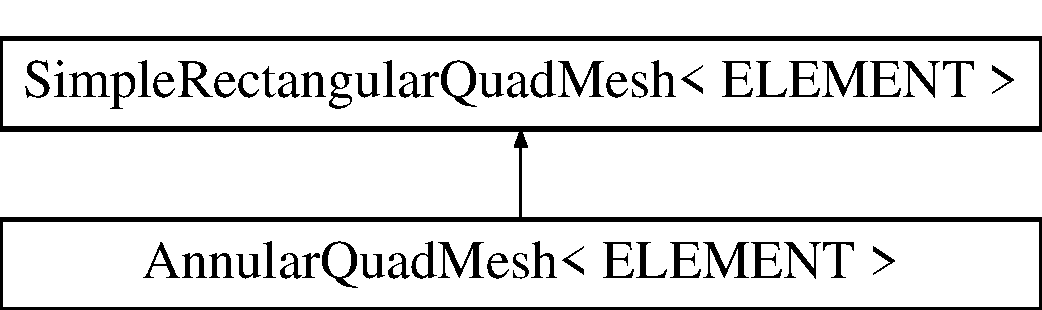
\includegraphics[height=2.000000cm]{classAnnularQuadMesh}
\end{center}
\end{figure}
\subsection*{Public Member Functions}
\begin{DoxyCompactItemize}
\item 
\hyperlink{classAnnularQuadMesh_acf01203e48fdee730b6c194bf538177c}{Annular\+Quad\+Mesh} (const unsigned \&n\+\_\+r, const unsigned \&n\+\_\+phi, const double \&r\+\_\+min, const double \&r\+\_\+max, const double \&phi\+\_\+min, const double \&phi\+\_\+max)
\end{DoxyCompactItemize}


\subsection{Detailed Description}
\subsubsection*{template$<$class E\+L\+E\+M\+E\+NT$>$\newline
class Annular\+Quad\+Mesh$<$ E\+L\+E\+M\+E\+N\+T $>$}



Definition at line 59 of file sphere\+\_\+scattering.\+cc.



\subsection{Constructor \& Destructor Documentation}
\mbox{\Hypertarget{classAnnularQuadMesh_acf01203e48fdee730b6c194bf538177c}\label{classAnnularQuadMesh_acf01203e48fdee730b6c194bf538177c}} 
\index{Annular\+Quad\+Mesh@{Annular\+Quad\+Mesh}!Annular\+Quad\+Mesh@{Annular\+Quad\+Mesh}}
\index{Annular\+Quad\+Mesh@{Annular\+Quad\+Mesh}!Annular\+Quad\+Mesh@{Annular\+Quad\+Mesh}}
\subsubsection{\texorpdfstring{Annular\+Quad\+Mesh()}{AnnularQuadMesh()}}
{\footnotesize\ttfamily template$<$class E\+L\+E\+M\+E\+NT$>$ \\
\hyperlink{classAnnularQuadMesh}{Annular\+Quad\+Mesh}$<$ E\+L\+E\+M\+E\+NT $>$\+::\hyperlink{classAnnularQuadMesh}{Annular\+Quad\+Mesh} (\begin{DoxyParamCaption}\item[{const unsigned \&}]{n\+\_\+r,  }\item[{const unsigned \&}]{n\+\_\+phi,  }\item[{const double \&}]{r\+\_\+min,  }\item[{const double \&}]{r\+\_\+max,  }\item[{const double \&}]{phi\+\_\+min,  }\item[{const double \&}]{phi\+\_\+max }\end{DoxyParamCaption})\hspace{0.3cm}{\ttfamily [inline]}}



Definition at line 69 of file sphere\+\_\+scattering.\+cc.



The documentation for this class was generated from the following file\+:\begin{DoxyCompactItemize}
\item 
\hyperlink{sphere__scattering_8cc}{sphere\+\_\+scattering.\+cc}\end{DoxyCompactItemize}

\hypertarget{classFourierDecomposedHelmholtzProblem}{}\section{Fourier\+Decomposed\+Helmholtz\+Problem$<$ E\+L\+E\+M\+E\+NT $>$ Class Template Reference}
\label{classFourierDecomposedHelmholtzProblem}\index{Fourier\+Decomposed\+Helmholtz\+Problem$<$ E\+L\+E\+M\+E\+N\+T $>$@{Fourier\+Decomposed\+Helmholtz\+Problem$<$ E\+L\+E\+M\+E\+N\+T $>$}}


Problem class.  


Inheritance diagram for Fourier\+Decomposed\+Helmholtz\+Problem$<$ E\+L\+E\+M\+E\+NT $>$\+:\begin{figure}[H]
\begin{center}
\leavevmode
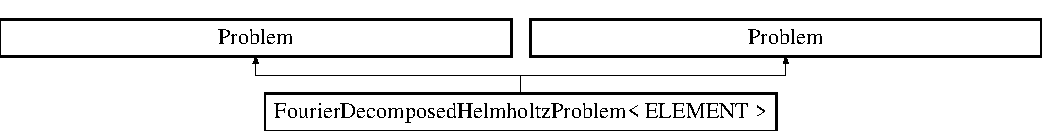
\includegraphics[height=1.766562cm]{classFourierDecomposedHelmholtzProblem}
\end{center}
\end{figure}
\subsection*{Public Member Functions}
\begin{DoxyCompactItemize}
\item 
\hyperlink{classFourierDecomposedHelmholtzProblem_ab368ed8fe04d4e3db67d13bab9e7b52e}{Fourier\+Decomposed\+Helmholtz\+Problem} ()
\begin{DoxyCompactList}\small\item\em Constructor. \end{DoxyCompactList}\item 
\hyperlink{classFourierDecomposedHelmholtzProblem_a03174fa5a35b7c38f08f91bcd2a80c20}{$\sim$\+Fourier\+Decomposed\+Helmholtz\+Problem} ()
\begin{DoxyCompactList}\small\item\em Destructor (empty) \end{DoxyCompactList}\item 
void \hyperlink{classFourierDecomposedHelmholtzProblem_a82ef5a969f4404fc1acb35c38c800ce6}{actions\+\_\+before\+\_\+newton\+\_\+solve} ()
\begin{DoxyCompactList}\small\item\em Update the problem specs before solve (empty) \end{DoxyCompactList}\item 
void \hyperlink{classFourierDecomposedHelmholtzProblem_a5a37ba3fcf8563764f80108c9a657929}{actions\+\_\+after\+\_\+newton\+\_\+solve} ()
\begin{DoxyCompactList}\small\item\em Update the problem after solve (empty) \end{DoxyCompactList}\item 
void \hyperlink{classFourierDecomposedHelmholtzProblem_a893efb01f8f1d254315201121766d882}{doc\+\_\+solution} (Doc\+Info \&doc\+\_\+info)
\begin{DoxyCompactList}\small\item\em Doc the solution. Doc\+Info object stores flags/labels for where the output gets written to. \end{DoxyCompactList}\item 
void \hyperlink{classFourierDecomposedHelmholtzProblem_ae80673ef299e4935ddcac177ed919da3}{actions\+\_\+before\+\_\+newton\+\_\+convergence\+\_\+check} ()
\begin{DoxyCompactList}\small\item\em Recompute gamma integral before checking Newton residuals. \end{DoxyCompactList}\item 
void \hyperlink{classFourierDecomposedHelmholtzProblem_ac4f3f737660b11e8762a61bca999eb0f}{check\+\_\+gamma} (Doc\+Info \&doc\+\_\+info)
\begin{DoxyCompactList}\small\item\em Check gamma computation. \end{DoxyCompactList}\item 
\hyperlink{classFourierDecomposedHelmholtzProblem_ab368ed8fe04d4e3db67d13bab9e7b52e}{Fourier\+Decomposed\+Helmholtz\+Problem} ()
\begin{DoxyCompactList}\small\item\em Constructor. \end{DoxyCompactList}\item 
\hyperlink{classFourierDecomposedHelmholtzProblem_a03174fa5a35b7c38f08f91bcd2a80c20}{$\sim$\+Fourier\+Decomposed\+Helmholtz\+Problem} ()
\begin{DoxyCompactList}\small\item\em Destructor (empty) \end{DoxyCompactList}\item 
void \hyperlink{classFourierDecomposedHelmholtzProblem_a82ef5a969f4404fc1acb35c38c800ce6}{actions\+\_\+before\+\_\+newton\+\_\+solve} ()
\begin{DoxyCompactList}\small\item\em Update the problem specs before solve (empty) \end{DoxyCompactList}\item 
void \hyperlink{classFourierDecomposedHelmholtzProblem_a5a37ba3fcf8563764f80108c9a657929}{actions\+\_\+after\+\_\+newton\+\_\+solve} ()
\begin{DoxyCompactList}\small\item\em Update the problem after solve (empty) \end{DoxyCompactList}\item 
void \hyperlink{classFourierDecomposedHelmholtzProblem_a893efb01f8f1d254315201121766d882}{doc\+\_\+solution} (Doc\+Info \&doc\+\_\+info)
\begin{DoxyCompactList}\small\item\em Doc the solution. Doc\+Info object stores flags/labels for where the output gets written to. \end{DoxyCompactList}\item 
void \hyperlink{classFourierDecomposedHelmholtzProblem_ae80673ef299e4935ddcac177ed919da3}{actions\+\_\+before\+\_\+newton\+\_\+convergence\+\_\+check} ()
\begin{DoxyCompactList}\small\item\em Recompute gamma integral before checking Newton residuals. \end{DoxyCompactList}\item 
void \hyperlink{classFourierDecomposedHelmholtzProblem_acbc6f3c692463e5a098ccec7fe9029c1}{actions\+\_\+before\+\_\+adapt} ()
\begin{DoxyCompactList}\small\item\em Actions before adapt\+: Wipe the mesh of prescribed flux elements. \end{DoxyCompactList}\item 
void \hyperlink{classFourierDecomposedHelmholtzProblem_a3258e3817d8747aac0409eca1a24d14b}{actions\+\_\+after\+\_\+adapt} ()
\begin{DoxyCompactList}\small\item\em Actions after adapt\+: Rebuild the mesh of prescribed flux elements. \end{DoxyCompactList}\item 
void \hyperlink{classFourierDecomposedHelmholtzProblem_ac4f3f737660b11e8762a61bca999eb0f}{check\+\_\+gamma} (Doc\+Info \&doc\+\_\+info)
\begin{DoxyCompactList}\small\item\em Check gamma computation. \end{DoxyCompactList}\end{DoxyCompactItemize}
\subsection*{Private Member Functions}
\begin{DoxyCompactItemize}
\item 
void \hyperlink{classFourierDecomposedHelmholtzProblem_a359d402bb4aed7d83973248d82085efb}{create\+\_\+outer\+\_\+bc\+\_\+elements} ()
\begin{DoxyCompactList}\small\item\em Create BC elements on outer boundary. \end{DoxyCompactList}\item 
void \hyperlink{classFourierDecomposedHelmholtzProblem_a81d64611f2de2492cec6b0621d8124b0}{create\+\_\+flux\+\_\+elements\+\_\+on\+\_\+inner\+\_\+boundary} ()
\begin{DoxyCompactList}\small\item\em Create flux elements on inner boundary. \end{DoxyCompactList}\item 
void \hyperlink{classFourierDecomposedHelmholtzProblem_a359d402bb4aed7d83973248d82085efb}{create\+\_\+outer\+\_\+bc\+\_\+elements} ()
\begin{DoxyCompactList}\small\item\em Create BC elements on outer boundary. \end{DoxyCompactList}\item 
void \hyperlink{classFourierDecomposedHelmholtzProblem_a81d64611f2de2492cec6b0621d8124b0}{create\+\_\+flux\+\_\+elements\+\_\+on\+\_\+inner\+\_\+boundary} ()
\begin{DoxyCompactList}\small\item\em Create flux elements on inner boundary. \end{DoxyCompactList}\item 
void \hyperlink{classFourierDecomposedHelmholtzProblem_aa2c19a495d042fbeca1e226e2ff73080}{delete\+\_\+face\+\_\+elements} (Mesh $\ast$const \&boundary\+\_\+mesh\+\_\+pt)
\begin{DoxyCompactList}\small\item\em Delete boundary face elements and wipe the surface mesh. \end{DoxyCompactList}\end{DoxyCompactItemize}
\subsection*{Private Attributes}
\begin{DoxyCompactItemize}
\item 
\hyperlink{classAnnularQuadMesh}{Annular\+Quad\+Mesh}$<$ E\+L\+E\+M\+E\+NT $>$ $\ast$ \hyperlink{classFourierDecomposedHelmholtzProblem_ad5927e4a2156e96c55ebce044c6f9653}{Bulk\+\_\+mesh\+\_\+pt}
\begin{DoxyCompactList}\small\item\em Pointer to bulk mesh. \end{DoxyCompactList}\item 
Fourier\+Decomposed\+Helmholtz\+Dt\+N\+Mesh$<$ E\+L\+E\+M\+E\+NT $>$ $\ast$ \hyperlink{classFourierDecomposedHelmholtzProblem_ab7aafa9c0ab982d9e1fdc31d802d309b}{Helmholtz\+\_\+outer\+\_\+boundary\+\_\+mesh\+\_\+pt}
\begin{DoxyCompactList}\small\item\em Pointer to mesh containing the DtN boundary condition elements. \end{DoxyCompactList}\item 
Mesh $\ast$ \hyperlink{classFourierDecomposedHelmholtzProblem_a3ecc5a3fc3407de8985ed9a61402f2f0}{Helmholtz\+\_\+inner\+\_\+boundary\+\_\+mesh\+\_\+pt}
\begin{DoxyCompactList}\small\item\em Mesh of face elements that apply the prescribed flux on the inner boundary. \end{DoxyCompactList}\item 
Refineable\+Triangle\+Mesh$<$ E\+L\+E\+M\+E\+NT $>$ $\ast$ \hyperlink{classFourierDecomposedHelmholtzProblem_a48a453a291906bbc152c21e2151bcb0c}{Bulk\+\_\+mesh\+\_\+pt}
\begin{DoxyCompactList}\small\item\em Pointer to the \char`\"{}bulk\char`\"{} mesh. \end{DoxyCompactList}\item 
Triangle\+Mesh$<$ E\+L\+E\+M\+E\+NT $>$ $\ast$ \hyperlink{classFourierDecomposedHelmholtzProblem_aa7ce7dc89eae3e8a753d3b8f0d71dbc4}{Bulk\+\_\+mesh\+\_\+pt}
\begin{DoxyCompactList}\small\item\em Pointer to the \char`\"{}bulk\char`\"{} mesh. \end{DoxyCompactList}\item 
ofstream \hyperlink{classFourierDecomposedHelmholtzProblem_ab9786130005c43637f8b305c2becc555}{Trace\+\_\+file}
\begin{DoxyCompactList}\small\item\em Trace file. \end{DoxyCompactList}\end{DoxyCompactItemize}


\subsection{Detailed Description}
\subsubsection*{template$<$class E\+L\+E\+M\+E\+NT$>$\newline
class Fourier\+Decomposed\+Helmholtz\+Problem$<$ E\+L\+E\+M\+E\+N\+T $>$}

Problem class. 

Definition at line 383 of file sphere\+\_\+scattering.\+cc.



\subsection{Constructor \& Destructor Documentation}
\mbox{\Hypertarget{classFourierDecomposedHelmholtzProblem_ab368ed8fe04d4e3db67d13bab9e7b52e}\label{classFourierDecomposedHelmholtzProblem_ab368ed8fe04d4e3db67d13bab9e7b52e}} 
\index{Fourier\+Decomposed\+Helmholtz\+Problem@{Fourier\+Decomposed\+Helmholtz\+Problem}!Fourier\+Decomposed\+Helmholtz\+Problem@{Fourier\+Decomposed\+Helmholtz\+Problem}}
\index{Fourier\+Decomposed\+Helmholtz\+Problem@{Fourier\+Decomposed\+Helmholtz\+Problem}!Fourier\+Decomposed\+Helmholtz\+Problem@{Fourier\+Decomposed\+Helmholtz\+Problem}}
\subsubsection{\texorpdfstring{Fourier\+Decomposed\+Helmholtz\+Problem()}{FourierDecomposedHelmholtzProblem()}\hspace{0.1cm}{\footnotesize\ttfamily [1/2]}}
{\footnotesize\ttfamily template$<$class E\+L\+E\+M\+E\+NT $>$ \\
\hyperlink{classFourierDecomposedHelmholtzProblem}{Fourier\+Decomposed\+Helmholtz\+Problem}$<$ E\+L\+E\+M\+E\+NT $>$\+::\hyperlink{classFourierDecomposedHelmholtzProblem}{Fourier\+Decomposed\+Helmholtz\+Problem} (\begin{DoxyParamCaption}{ }\end{DoxyParamCaption})}



Constructor. 

Constructor for Fourier-\/decomposed Helmholtz problem. 

Definition at line 441 of file sphere\+\_\+scattering.\+cc.



References Problem\+Parameters\+::\+El\+\_\+multiplier, Problem\+Parameters\+::\+K\+\_\+squared, Problem\+Parameters\+::\+N\+\_\+fourier, and Problem\+Parameters\+::\+Nterms\+\_\+for\+\_\+\+DtN.



Referenced by Fourier\+Decomposed\+Helmholtz\+Problem$<$ E\+L\+E\+M\+E\+N\+T $>$\+::actions\+\_\+after\+\_\+adapt().

\mbox{\Hypertarget{classFourierDecomposedHelmholtzProblem_a03174fa5a35b7c38f08f91bcd2a80c20}\label{classFourierDecomposedHelmholtzProblem_a03174fa5a35b7c38f08f91bcd2a80c20}} 
\index{Fourier\+Decomposed\+Helmholtz\+Problem@{Fourier\+Decomposed\+Helmholtz\+Problem}!````~Fourier\+Decomposed\+Helmholtz\+Problem@{$\sim$\+Fourier\+Decomposed\+Helmholtz\+Problem}}
\index{````~Fourier\+Decomposed\+Helmholtz\+Problem@{$\sim$\+Fourier\+Decomposed\+Helmholtz\+Problem}!Fourier\+Decomposed\+Helmholtz\+Problem@{Fourier\+Decomposed\+Helmholtz\+Problem}}
\subsubsection{\texorpdfstring{$\sim$\+Fourier\+Decomposed\+Helmholtz\+Problem()}{~FourierDecomposedHelmholtzProblem()}\hspace{0.1cm}{\footnotesize\ttfamily [1/2]}}
{\footnotesize\ttfamily template$<$class E\+L\+E\+M\+E\+NT$>$ \\
\hyperlink{classFourierDecomposedHelmholtzProblem}{Fourier\+Decomposed\+Helmholtz\+Problem}$<$ E\+L\+E\+M\+E\+NT $>$\+::$\sim$\hyperlink{classFourierDecomposedHelmholtzProblem}{Fourier\+Decomposed\+Helmholtz\+Problem} (\begin{DoxyParamCaption}{ }\end{DoxyParamCaption})\hspace{0.3cm}{\ttfamily [inline]}}



Destructor (empty) 



Definition at line 392 of file sphere\+\_\+scattering.\+cc.

\mbox{\Hypertarget{classFourierDecomposedHelmholtzProblem_ab368ed8fe04d4e3db67d13bab9e7b52e}\label{classFourierDecomposedHelmholtzProblem_ab368ed8fe04d4e3db67d13bab9e7b52e}} 
\index{Fourier\+Decomposed\+Helmholtz\+Problem@{Fourier\+Decomposed\+Helmholtz\+Problem}!Fourier\+Decomposed\+Helmholtz\+Problem@{Fourier\+Decomposed\+Helmholtz\+Problem}}
\index{Fourier\+Decomposed\+Helmholtz\+Problem@{Fourier\+Decomposed\+Helmholtz\+Problem}!Fourier\+Decomposed\+Helmholtz\+Problem@{Fourier\+Decomposed\+Helmholtz\+Problem}}
\subsubsection{\texorpdfstring{Fourier\+Decomposed\+Helmholtz\+Problem()}{FourierDecomposedHelmholtzProblem()}\hspace{0.1cm}{\footnotesize\ttfamily [2/2]}}
{\footnotesize\ttfamily template$<$class E\+L\+E\+M\+E\+NT$>$ \\
\hyperlink{classFourierDecomposedHelmholtzProblem}{Fourier\+Decomposed\+Helmholtz\+Problem}$<$ E\+L\+E\+M\+E\+NT $>$\+::\hyperlink{classFourierDecomposedHelmholtzProblem}{Fourier\+Decomposed\+Helmholtz\+Problem} (\begin{DoxyParamCaption}{ }\end{DoxyParamCaption})}



Constructor. 

\mbox{\Hypertarget{classFourierDecomposedHelmholtzProblem_a03174fa5a35b7c38f08f91bcd2a80c20}\label{classFourierDecomposedHelmholtzProblem_a03174fa5a35b7c38f08f91bcd2a80c20}} 
\index{Fourier\+Decomposed\+Helmholtz\+Problem@{Fourier\+Decomposed\+Helmholtz\+Problem}!````~Fourier\+Decomposed\+Helmholtz\+Problem@{$\sim$\+Fourier\+Decomposed\+Helmholtz\+Problem}}
\index{````~Fourier\+Decomposed\+Helmholtz\+Problem@{$\sim$\+Fourier\+Decomposed\+Helmholtz\+Problem}!Fourier\+Decomposed\+Helmholtz\+Problem@{Fourier\+Decomposed\+Helmholtz\+Problem}}
\subsubsection{\texorpdfstring{$\sim$\+Fourier\+Decomposed\+Helmholtz\+Problem()}{~FourierDecomposedHelmholtzProblem()}\hspace{0.1cm}{\footnotesize\ttfamily [2/2]}}
{\footnotesize\ttfamily template$<$class E\+L\+E\+M\+E\+NT$>$ \\
\hyperlink{classFourierDecomposedHelmholtzProblem}{Fourier\+Decomposed\+Helmholtz\+Problem}$<$ E\+L\+E\+M\+E\+NT $>$\+::$\sim$\hyperlink{classFourierDecomposedHelmholtzProblem}{Fourier\+Decomposed\+Helmholtz\+Problem} (\begin{DoxyParamCaption}{ }\end{DoxyParamCaption})\hspace{0.3cm}{\ttfamily [inline]}}



Destructor (empty) 



Definition at line 337 of file unstructured\+\_\+sphere\+\_\+scattering.\+cc.



\subsection{Member Function Documentation}
\mbox{\Hypertarget{classFourierDecomposedHelmholtzProblem_a3258e3817d8747aac0409eca1a24d14b}\label{classFourierDecomposedHelmholtzProblem_a3258e3817d8747aac0409eca1a24d14b}} 
\index{Fourier\+Decomposed\+Helmholtz\+Problem@{Fourier\+Decomposed\+Helmholtz\+Problem}!actions\+\_\+after\+\_\+adapt@{actions\+\_\+after\+\_\+adapt}}
\index{actions\+\_\+after\+\_\+adapt@{actions\+\_\+after\+\_\+adapt}!Fourier\+Decomposed\+Helmholtz\+Problem@{Fourier\+Decomposed\+Helmholtz\+Problem}}
\subsubsection{\texorpdfstring{actions\+\_\+after\+\_\+adapt()}{actions\_after\_adapt()}}
{\footnotesize\ttfamily template$<$class E\+L\+E\+M\+E\+NT $>$ \\
void \hyperlink{classFourierDecomposedHelmholtzProblem}{Fourier\+Decomposed\+Helmholtz\+Problem}$<$ E\+L\+E\+M\+E\+NT $>$\+::actions\+\_\+after\+\_\+adapt (\begin{DoxyParamCaption}{ }\end{DoxyParamCaption})}



Actions after adapt\+: Rebuild the mesh of prescribed flux elements. 

Actions after adapt\+: Rebuild the face element meshes. 

Definition at line 441 of file unstructured\+\_\+sphere\+\_\+scattering.\+cc.



References Fourier\+Decomposed\+Helmholtz\+Problem$<$ E\+L\+E\+M\+E\+N\+T $>$\+::check\+\_\+gamma(), Fourier\+Decomposed\+Helmholtz\+Problem$<$ E\+L\+E\+M\+E\+N\+T $>$\+::create\+\_\+flux\+\_\+elements\+\_\+on\+\_\+inner\+\_\+boundary(), Fourier\+Decomposed\+Helmholtz\+Problem$<$ E\+L\+E\+M\+E\+N\+T $>$\+::create\+\_\+outer\+\_\+bc\+\_\+elements(), Fourier\+Decomposed\+Helmholtz\+Problem$<$ E\+L\+E\+M\+E\+N\+T $>$\+::doc\+\_\+solution(), Problem\+Parameters\+::exact\+\_\+minus\+\_\+dudr(), Fourier\+Decomposed\+Helmholtz\+Problem$<$ E\+L\+E\+M\+E\+N\+T $>$\+::\+Fourier\+Decomposed\+Helmholtz\+Problem(), Problem\+Parameters\+::get\+\_\+exact\+\_\+u(), Problem\+Parameters\+::\+K\+\_\+squared, Problem\+Parameters\+::\+N\+\_\+fourier, and Problem\+Parameters\+::\+Nterms\+\_\+for\+\_\+\+DtN.

\mbox{\Hypertarget{classFourierDecomposedHelmholtzProblem_a5a37ba3fcf8563764f80108c9a657929}\label{classFourierDecomposedHelmholtzProblem_a5a37ba3fcf8563764f80108c9a657929}} 
\index{Fourier\+Decomposed\+Helmholtz\+Problem@{Fourier\+Decomposed\+Helmholtz\+Problem}!actions\+\_\+after\+\_\+newton\+\_\+solve@{actions\+\_\+after\+\_\+newton\+\_\+solve}}
\index{actions\+\_\+after\+\_\+newton\+\_\+solve@{actions\+\_\+after\+\_\+newton\+\_\+solve}!Fourier\+Decomposed\+Helmholtz\+Problem@{Fourier\+Decomposed\+Helmholtz\+Problem}}
\subsubsection{\texorpdfstring{actions\+\_\+after\+\_\+newton\+\_\+solve()}{actions\_after\_newton\_solve()}\hspace{0.1cm}{\footnotesize\ttfamily [1/2]}}
{\footnotesize\ttfamily template$<$class E\+L\+E\+M\+E\+NT$>$ \\
void \hyperlink{classFourierDecomposedHelmholtzProblem}{Fourier\+Decomposed\+Helmholtz\+Problem}$<$ E\+L\+E\+M\+E\+NT $>$\+::actions\+\_\+after\+\_\+newton\+\_\+solve (\begin{DoxyParamCaption}{ }\end{DoxyParamCaption})\hspace{0.3cm}{\ttfamily [inline]}}



Update the problem after solve (empty) 



Definition at line 343 of file unstructured\+\_\+sphere\+\_\+scattering.\+cc.

\mbox{\Hypertarget{classFourierDecomposedHelmholtzProblem_a5a37ba3fcf8563764f80108c9a657929}\label{classFourierDecomposedHelmholtzProblem_a5a37ba3fcf8563764f80108c9a657929}} 
\index{Fourier\+Decomposed\+Helmholtz\+Problem@{Fourier\+Decomposed\+Helmholtz\+Problem}!actions\+\_\+after\+\_\+newton\+\_\+solve@{actions\+\_\+after\+\_\+newton\+\_\+solve}}
\index{actions\+\_\+after\+\_\+newton\+\_\+solve@{actions\+\_\+after\+\_\+newton\+\_\+solve}!Fourier\+Decomposed\+Helmholtz\+Problem@{Fourier\+Decomposed\+Helmholtz\+Problem}}
\subsubsection{\texorpdfstring{actions\+\_\+after\+\_\+newton\+\_\+solve()}{actions\_after\_newton\_solve()}\hspace{0.1cm}{\footnotesize\ttfamily [2/2]}}
{\footnotesize\ttfamily template$<$class E\+L\+E\+M\+E\+NT$>$ \\
void \hyperlink{classFourierDecomposedHelmholtzProblem}{Fourier\+Decomposed\+Helmholtz\+Problem}$<$ E\+L\+E\+M\+E\+NT $>$\+::actions\+\_\+after\+\_\+newton\+\_\+solve (\begin{DoxyParamCaption}{ }\end{DoxyParamCaption})\hspace{0.3cm}{\ttfamily [inline]}}



Update the problem after solve (empty) 



Definition at line 398 of file sphere\+\_\+scattering.\+cc.

\mbox{\Hypertarget{classFourierDecomposedHelmholtzProblem_acbc6f3c692463e5a098ccec7fe9029c1}\label{classFourierDecomposedHelmholtzProblem_acbc6f3c692463e5a098ccec7fe9029c1}} 
\index{Fourier\+Decomposed\+Helmholtz\+Problem@{Fourier\+Decomposed\+Helmholtz\+Problem}!actions\+\_\+before\+\_\+adapt@{actions\+\_\+before\+\_\+adapt}}
\index{actions\+\_\+before\+\_\+adapt@{actions\+\_\+before\+\_\+adapt}!Fourier\+Decomposed\+Helmholtz\+Problem@{Fourier\+Decomposed\+Helmholtz\+Problem}}
\subsubsection{\texorpdfstring{actions\+\_\+before\+\_\+adapt()}{actions\_before\_adapt()}}
{\footnotesize\ttfamily template$<$class E\+L\+E\+M\+E\+NT $>$ \\
void \hyperlink{classFourierDecomposedHelmholtzProblem}{Fourier\+Decomposed\+Helmholtz\+Problem}$<$ E\+L\+E\+M\+E\+NT $>$\+::actions\+\_\+before\+\_\+adapt (\begin{DoxyParamCaption}{ }\end{DoxyParamCaption})}



Actions before adapt\+: Wipe the mesh of prescribed flux elements. 

Actions before adapt\+: Wipe the mesh of face elements. 

Definition at line 422 of file unstructured\+\_\+sphere\+\_\+scattering.\+cc.

\mbox{\Hypertarget{classFourierDecomposedHelmholtzProblem_ae80673ef299e4935ddcac177ed919da3}\label{classFourierDecomposedHelmholtzProblem_ae80673ef299e4935ddcac177ed919da3}} 
\index{Fourier\+Decomposed\+Helmholtz\+Problem@{Fourier\+Decomposed\+Helmholtz\+Problem}!actions\+\_\+before\+\_\+newton\+\_\+convergence\+\_\+check@{actions\+\_\+before\+\_\+newton\+\_\+convergence\+\_\+check}}
\index{actions\+\_\+before\+\_\+newton\+\_\+convergence\+\_\+check@{actions\+\_\+before\+\_\+newton\+\_\+convergence\+\_\+check}!Fourier\+Decomposed\+Helmholtz\+Problem@{Fourier\+Decomposed\+Helmholtz\+Problem}}
\subsubsection{\texorpdfstring{actions\+\_\+before\+\_\+newton\+\_\+convergence\+\_\+check()}{actions\_before\_newton\_convergence\_check()}\hspace{0.1cm}{\footnotesize\ttfamily [1/2]}}
{\footnotesize\ttfamily template$<$class E\+L\+E\+M\+E\+NT$>$ \\
void \hyperlink{classFourierDecomposedHelmholtzProblem}{Fourier\+Decomposed\+Helmholtz\+Problem}$<$ E\+L\+E\+M\+E\+NT $>$\+::actions\+\_\+before\+\_\+newton\+\_\+convergence\+\_\+check (\begin{DoxyParamCaption}{ }\end{DoxyParamCaption})\hspace{0.3cm}{\ttfamily [inline]}}



Recompute gamma integral before checking Newton residuals. 



Definition at line 350 of file unstructured\+\_\+sphere\+\_\+scattering.\+cc.

\mbox{\Hypertarget{classFourierDecomposedHelmholtzProblem_ae80673ef299e4935ddcac177ed919da3}\label{classFourierDecomposedHelmholtzProblem_ae80673ef299e4935ddcac177ed919da3}} 
\index{Fourier\+Decomposed\+Helmholtz\+Problem@{Fourier\+Decomposed\+Helmholtz\+Problem}!actions\+\_\+before\+\_\+newton\+\_\+convergence\+\_\+check@{actions\+\_\+before\+\_\+newton\+\_\+convergence\+\_\+check}}
\index{actions\+\_\+before\+\_\+newton\+\_\+convergence\+\_\+check@{actions\+\_\+before\+\_\+newton\+\_\+convergence\+\_\+check}!Fourier\+Decomposed\+Helmholtz\+Problem@{Fourier\+Decomposed\+Helmholtz\+Problem}}
\subsubsection{\texorpdfstring{actions\+\_\+before\+\_\+newton\+\_\+convergence\+\_\+check()}{actions\_before\_newton\_convergence\_check()}\hspace{0.1cm}{\footnotesize\ttfamily [2/2]}}
{\footnotesize\ttfamily template$<$class E\+L\+E\+M\+E\+NT$>$ \\
void \hyperlink{classFourierDecomposedHelmholtzProblem}{Fourier\+Decomposed\+Helmholtz\+Problem}$<$ E\+L\+E\+M\+E\+NT $>$\+::actions\+\_\+before\+\_\+newton\+\_\+convergence\+\_\+check (\begin{DoxyParamCaption}{ }\end{DoxyParamCaption})\hspace{0.3cm}{\ttfamily [inline]}}



Recompute gamma integral before checking Newton residuals. 



Definition at line 405 of file sphere\+\_\+scattering.\+cc.

\mbox{\Hypertarget{classFourierDecomposedHelmholtzProblem_a82ef5a969f4404fc1acb35c38c800ce6}\label{classFourierDecomposedHelmholtzProblem_a82ef5a969f4404fc1acb35c38c800ce6}} 
\index{Fourier\+Decomposed\+Helmholtz\+Problem@{Fourier\+Decomposed\+Helmholtz\+Problem}!actions\+\_\+before\+\_\+newton\+\_\+solve@{actions\+\_\+before\+\_\+newton\+\_\+solve}}
\index{actions\+\_\+before\+\_\+newton\+\_\+solve@{actions\+\_\+before\+\_\+newton\+\_\+solve}!Fourier\+Decomposed\+Helmholtz\+Problem@{Fourier\+Decomposed\+Helmholtz\+Problem}}
\subsubsection{\texorpdfstring{actions\+\_\+before\+\_\+newton\+\_\+solve()}{actions\_before\_newton\_solve()}\hspace{0.1cm}{\footnotesize\ttfamily [1/2]}}
{\footnotesize\ttfamily template$<$class E\+L\+E\+M\+E\+NT$>$ \\
void \hyperlink{classFourierDecomposedHelmholtzProblem}{Fourier\+Decomposed\+Helmholtz\+Problem}$<$ E\+L\+E\+M\+E\+NT $>$\+::actions\+\_\+before\+\_\+newton\+\_\+solve (\begin{DoxyParamCaption}{ }\end{DoxyParamCaption})\hspace{0.3cm}{\ttfamily [inline]}}



Update the problem specs before solve (empty) 



Definition at line 340 of file unstructured\+\_\+sphere\+\_\+scattering.\+cc.

\mbox{\Hypertarget{classFourierDecomposedHelmholtzProblem_a82ef5a969f4404fc1acb35c38c800ce6}\label{classFourierDecomposedHelmholtzProblem_a82ef5a969f4404fc1acb35c38c800ce6}} 
\index{Fourier\+Decomposed\+Helmholtz\+Problem@{Fourier\+Decomposed\+Helmholtz\+Problem}!actions\+\_\+before\+\_\+newton\+\_\+solve@{actions\+\_\+before\+\_\+newton\+\_\+solve}}
\index{actions\+\_\+before\+\_\+newton\+\_\+solve@{actions\+\_\+before\+\_\+newton\+\_\+solve}!Fourier\+Decomposed\+Helmholtz\+Problem@{Fourier\+Decomposed\+Helmholtz\+Problem}}
\subsubsection{\texorpdfstring{actions\+\_\+before\+\_\+newton\+\_\+solve()}{actions\_before\_newton\_solve()}\hspace{0.1cm}{\footnotesize\ttfamily [2/2]}}
{\footnotesize\ttfamily template$<$class E\+L\+E\+M\+E\+NT$>$ \\
void \hyperlink{classFourierDecomposedHelmholtzProblem}{Fourier\+Decomposed\+Helmholtz\+Problem}$<$ E\+L\+E\+M\+E\+NT $>$\+::actions\+\_\+before\+\_\+newton\+\_\+solve (\begin{DoxyParamCaption}{ }\end{DoxyParamCaption})\hspace{0.3cm}{\ttfamily [inline]}}



Update the problem specs before solve (empty) 



Definition at line 395 of file sphere\+\_\+scattering.\+cc.

\mbox{\Hypertarget{classFourierDecomposedHelmholtzProblem_ac4f3f737660b11e8762a61bca999eb0f}\label{classFourierDecomposedHelmholtzProblem_ac4f3f737660b11e8762a61bca999eb0f}} 
\index{Fourier\+Decomposed\+Helmholtz\+Problem@{Fourier\+Decomposed\+Helmholtz\+Problem}!check\+\_\+gamma@{check\+\_\+gamma}}
\index{check\+\_\+gamma@{check\+\_\+gamma}!Fourier\+Decomposed\+Helmholtz\+Problem@{Fourier\+Decomposed\+Helmholtz\+Problem}}
\subsubsection{\texorpdfstring{check\+\_\+gamma()}{check\_gamma()}\hspace{0.1cm}{\footnotesize\ttfamily [1/2]}}
{\footnotesize\ttfamily template$<$class E\+L\+E\+M\+E\+NT$>$ \\
void \hyperlink{classFourierDecomposedHelmholtzProblem}{Fourier\+Decomposed\+Helmholtz\+Problem}$<$ E\+L\+E\+M\+E\+NT $>$\+::check\+\_\+gamma (\begin{DoxyParamCaption}\item[{Doc\+Info \&}]{doc\+\_\+info }\end{DoxyParamCaption})}



Check gamma computation. 

\mbox{\Hypertarget{classFourierDecomposedHelmholtzProblem_ac4f3f737660b11e8762a61bca999eb0f}\label{classFourierDecomposedHelmholtzProblem_ac4f3f737660b11e8762a61bca999eb0f}} 
\index{Fourier\+Decomposed\+Helmholtz\+Problem@{Fourier\+Decomposed\+Helmholtz\+Problem}!check\+\_\+gamma@{check\+\_\+gamma}}
\index{check\+\_\+gamma@{check\+\_\+gamma}!Fourier\+Decomposed\+Helmholtz\+Problem@{Fourier\+Decomposed\+Helmholtz\+Problem}}
\subsubsection{\texorpdfstring{check\+\_\+gamma()}{check\_gamma()}\hspace{0.1cm}{\footnotesize\ttfamily [2/2]}}
{\footnotesize\ttfamily template$<$class E\+L\+E\+M\+E\+NT $>$ \\
void \hyperlink{classFourierDecomposedHelmholtzProblem}{Fourier\+Decomposed\+Helmholtz\+Problem}$<$ E\+L\+E\+M\+E\+NT $>$\+::check\+\_\+gamma (\begin{DoxyParamCaption}\item[{Doc\+Info \&}]{doc\+\_\+info }\end{DoxyParamCaption})}



Check gamma computation. 

Check gamma computation\+: $ \gamma = -du/dn $. 

Definition at line 509 of file sphere\+\_\+scattering.\+cc.



References Problem\+Parameters\+::exact\+\_\+minus\+\_\+dudr().



Referenced by Fourier\+Decomposed\+Helmholtz\+Problem$<$ E\+L\+E\+M\+E\+N\+T $>$\+::actions\+\_\+after\+\_\+adapt().

\mbox{\Hypertarget{classFourierDecomposedHelmholtzProblem_a81d64611f2de2492cec6b0621d8124b0}\label{classFourierDecomposedHelmholtzProblem_a81d64611f2de2492cec6b0621d8124b0}} 
\index{Fourier\+Decomposed\+Helmholtz\+Problem@{Fourier\+Decomposed\+Helmholtz\+Problem}!create\+\_\+flux\+\_\+elements\+\_\+on\+\_\+inner\+\_\+boundary@{create\+\_\+flux\+\_\+elements\+\_\+on\+\_\+inner\+\_\+boundary}}
\index{create\+\_\+flux\+\_\+elements\+\_\+on\+\_\+inner\+\_\+boundary@{create\+\_\+flux\+\_\+elements\+\_\+on\+\_\+inner\+\_\+boundary}!Fourier\+Decomposed\+Helmholtz\+Problem@{Fourier\+Decomposed\+Helmholtz\+Problem}}
\subsubsection{\texorpdfstring{create\+\_\+flux\+\_\+elements\+\_\+on\+\_\+inner\+\_\+boundary()}{create\_flux\_elements\_on\_inner\_boundary()}\hspace{0.1cm}{\footnotesize\ttfamily [1/2]}}
{\footnotesize\ttfamily template$<$class E\+L\+E\+M\+E\+NT$>$ \\
void \hyperlink{classFourierDecomposedHelmholtzProblem}{Fourier\+Decomposed\+Helmholtz\+Problem}$<$ E\+L\+E\+M\+E\+NT $>$\+::create\+\_\+flux\+\_\+elements\+\_\+on\+\_\+inner\+\_\+boundary (\begin{DoxyParamCaption}{ }\end{DoxyParamCaption})\hspace{0.3cm}{\ttfamily [private]}}



Create flux elements on inner boundary. 

\mbox{\Hypertarget{classFourierDecomposedHelmholtzProblem_a81d64611f2de2492cec6b0621d8124b0}\label{classFourierDecomposedHelmholtzProblem_a81d64611f2de2492cec6b0621d8124b0}} 
\index{Fourier\+Decomposed\+Helmholtz\+Problem@{Fourier\+Decomposed\+Helmholtz\+Problem}!create\+\_\+flux\+\_\+elements\+\_\+on\+\_\+inner\+\_\+boundary@{create\+\_\+flux\+\_\+elements\+\_\+on\+\_\+inner\+\_\+boundary}}
\index{create\+\_\+flux\+\_\+elements\+\_\+on\+\_\+inner\+\_\+boundary@{create\+\_\+flux\+\_\+elements\+\_\+on\+\_\+inner\+\_\+boundary}!Fourier\+Decomposed\+Helmholtz\+Problem@{Fourier\+Decomposed\+Helmholtz\+Problem}}
\subsubsection{\texorpdfstring{create\+\_\+flux\+\_\+elements\+\_\+on\+\_\+inner\+\_\+boundary()}{create\_flux\_elements\_on\_inner\_boundary()}\hspace{0.1cm}{\footnotesize\ttfamily [2/2]}}
{\footnotesize\ttfamily template$<$class E\+L\+E\+M\+E\+NT $>$ \\
void \hyperlink{classFourierDecomposedHelmholtzProblem}{Fourier\+Decomposed\+Helmholtz\+Problem}$<$ E\+L\+E\+M\+E\+NT $>$\+::create\+\_\+flux\+\_\+elements\+\_\+on\+\_\+inner\+\_\+boundary (\begin{DoxyParamCaption}{ }\end{DoxyParamCaption})\hspace{0.3cm}{\ttfamily [private]}}



Create flux elements on inner boundary. 



Definition at line 701 of file sphere\+\_\+scattering.\+cc.



References Problem\+Parameters\+::exact\+\_\+minus\+\_\+dudr().



Referenced by Fourier\+Decomposed\+Helmholtz\+Problem$<$ E\+L\+E\+M\+E\+N\+T $>$\+::actions\+\_\+after\+\_\+adapt(), and Fourier\+Decomposed\+Helmholtz\+Problem$<$ E\+L\+E\+M\+E\+N\+T $>$\+::create\+\_\+outer\+\_\+bc\+\_\+elements().

\mbox{\Hypertarget{classFourierDecomposedHelmholtzProblem_a359d402bb4aed7d83973248d82085efb}\label{classFourierDecomposedHelmholtzProblem_a359d402bb4aed7d83973248d82085efb}} 
\index{Fourier\+Decomposed\+Helmholtz\+Problem@{Fourier\+Decomposed\+Helmholtz\+Problem}!create\+\_\+outer\+\_\+bc\+\_\+elements@{create\+\_\+outer\+\_\+bc\+\_\+elements}}
\index{create\+\_\+outer\+\_\+bc\+\_\+elements@{create\+\_\+outer\+\_\+bc\+\_\+elements}!Fourier\+Decomposed\+Helmholtz\+Problem@{Fourier\+Decomposed\+Helmholtz\+Problem}}
\subsubsection{\texorpdfstring{create\+\_\+outer\+\_\+bc\+\_\+elements()}{create\_outer\_bc\_elements()}\hspace{0.1cm}{\footnotesize\ttfamily [1/2]}}
{\footnotesize\ttfamily template$<$class E\+L\+E\+M\+E\+NT$>$ \\
void \hyperlink{classFourierDecomposedHelmholtzProblem}{Fourier\+Decomposed\+Helmholtz\+Problem}$<$ E\+L\+E\+M\+E\+NT $>$\+::create\+\_\+outer\+\_\+bc\+\_\+elements (\begin{DoxyParamCaption}{ }\end{DoxyParamCaption})\hspace{0.3cm}{\ttfamily [private]}}



Create BC elements on outer boundary. 

\mbox{\Hypertarget{classFourierDecomposedHelmholtzProblem_a359d402bb4aed7d83973248d82085efb}\label{classFourierDecomposedHelmholtzProblem_a359d402bb4aed7d83973248d82085efb}} 
\index{Fourier\+Decomposed\+Helmholtz\+Problem@{Fourier\+Decomposed\+Helmholtz\+Problem}!create\+\_\+outer\+\_\+bc\+\_\+elements@{create\+\_\+outer\+\_\+bc\+\_\+elements}}
\index{create\+\_\+outer\+\_\+bc\+\_\+elements@{create\+\_\+outer\+\_\+bc\+\_\+elements}!Fourier\+Decomposed\+Helmholtz\+Problem@{Fourier\+Decomposed\+Helmholtz\+Problem}}
\subsubsection{\texorpdfstring{create\+\_\+outer\+\_\+bc\+\_\+elements()}{create\_outer\_bc\_elements()}\hspace{0.1cm}{\footnotesize\ttfamily [2/2]}}
{\footnotesize\ttfamily template$<$class E\+L\+E\+M\+E\+NT $>$ \\
void \hyperlink{classFourierDecomposedHelmholtzProblem}{Fourier\+Decomposed\+Helmholtz\+Problem}$<$ E\+L\+E\+M\+E\+NT $>$\+::create\+\_\+outer\+\_\+bc\+\_\+elements (\begin{DoxyParamCaption}{ }\end{DoxyParamCaption})\hspace{0.3cm}{\ttfamily [private]}}



Create BC elements on outer boundary. 



Definition at line 662 of file sphere\+\_\+scattering.\+cc.



References Fourier\+Decomposed\+Helmholtz\+Problem$<$ E\+L\+E\+M\+E\+N\+T $>$\+::create\+\_\+flux\+\_\+elements\+\_\+on\+\_\+inner\+\_\+boundary().



Referenced by Fourier\+Decomposed\+Helmholtz\+Problem$<$ E\+L\+E\+M\+E\+N\+T $>$\+::actions\+\_\+after\+\_\+adapt().

\mbox{\Hypertarget{classFourierDecomposedHelmholtzProblem_aa2c19a495d042fbeca1e226e2ff73080}\label{classFourierDecomposedHelmholtzProblem_aa2c19a495d042fbeca1e226e2ff73080}} 
\index{Fourier\+Decomposed\+Helmholtz\+Problem@{Fourier\+Decomposed\+Helmholtz\+Problem}!delete\+\_\+face\+\_\+elements@{delete\+\_\+face\+\_\+elements}}
\index{delete\+\_\+face\+\_\+elements@{delete\+\_\+face\+\_\+elements}!Fourier\+Decomposed\+Helmholtz\+Problem@{Fourier\+Decomposed\+Helmholtz\+Problem}}
\subsubsection{\texorpdfstring{delete\+\_\+face\+\_\+elements()}{delete\_face\_elements()}}
{\footnotesize\ttfamily template$<$class E\+L\+E\+M\+E\+NT$>$ \\
void \hyperlink{classFourierDecomposedHelmholtzProblem}{Fourier\+Decomposed\+Helmholtz\+Problem}$<$ E\+L\+E\+M\+E\+NT $>$\+::delete\+\_\+face\+\_\+elements (\begin{DoxyParamCaption}\item[{Mesh $\ast$const \&}]{boundary\+\_\+mesh\+\_\+pt }\end{DoxyParamCaption})\hspace{0.3cm}{\ttfamily [inline]}, {\ttfamily [private]}}



Delete boundary face elements and wipe the surface mesh. 



Definition at line 377 of file unstructured\+\_\+sphere\+\_\+scattering.\+cc.

\mbox{\Hypertarget{classFourierDecomposedHelmholtzProblem_a893efb01f8f1d254315201121766d882}\label{classFourierDecomposedHelmholtzProblem_a893efb01f8f1d254315201121766d882}} 
\index{Fourier\+Decomposed\+Helmholtz\+Problem@{Fourier\+Decomposed\+Helmholtz\+Problem}!doc\+\_\+solution@{doc\+\_\+solution}}
\index{doc\+\_\+solution@{doc\+\_\+solution}!Fourier\+Decomposed\+Helmholtz\+Problem@{Fourier\+Decomposed\+Helmholtz\+Problem}}
\subsubsection{\texorpdfstring{doc\+\_\+solution()}{doc\_solution()}\hspace{0.1cm}{\footnotesize\ttfamily [1/2]}}
{\footnotesize\ttfamily template$<$class E\+L\+E\+M\+E\+NT$>$ \\
void \hyperlink{classFourierDecomposedHelmholtzProblem}{Fourier\+Decomposed\+Helmholtz\+Problem}$<$ E\+L\+E\+M\+E\+NT $>$\+::doc\+\_\+solution (\begin{DoxyParamCaption}\item[{Doc\+Info \&}]{doc\+\_\+info }\end{DoxyParamCaption})}



Doc the solution. Doc\+Info object stores flags/labels for where the output gets written to. 

\mbox{\Hypertarget{classFourierDecomposedHelmholtzProblem_a893efb01f8f1d254315201121766d882}\label{classFourierDecomposedHelmholtzProblem_a893efb01f8f1d254315201121766d882}} 
\index{Fourier\+Decomposed\+Helmholtz\+Problem@{Fourier\+Decomposed\+Helmholtz\+Problem}!doc\+\_\+solution@{doc\+\_\+solution}}
\index{doc\+\_\+solution@{doc\+\_\+solution}!Fourier\+Decomposed\+Helmholtz\+Problem@{Fourier\+Decomposed\+Helmholtz\+Problem}}
\subsubsection{\texorpdfstring{doc\+\_\+solution()}{doc\_solution()}\hspace{0.1cm}{\footnotesize\ttfamily [2/2]}}
{\footnotesize\ttfamily template$<$class E\+L\+E\+M\+E\+NT $>$ \\
void \hyperlink{classFourierDecomposedHelmholtzProblem}{Fourier\+Decomposed\+Helmholtz\+Problem}$<$ E\+L\+E\+M\+E\+NT $>$\+::doc\+\_\+solution (\begin{DoxyParamCaption}\item[{Doc\+Info \&}]{doc\+\_\+info }\end{DoxyParamCaption})}



Doc the solution. Doc\+Info object stores flags/labels for where the output gets written to. 

Doc the solution\+: doc\+\_\+info contains labels/output directory etc. 

Definition at line 578 of file sphere\+\_\+scattering.\+cc.



References Problem\+Parameters\+::get\+\_\+exact\+\_\+u(), Problem\+Parameters\+::\+K\+\_\+squared, and Problem\+Parameters\+::\+N\+\_\+fourier.



Referenced by Fourier\+Decomposed\+Helmholtz\+Problem$<$ E\+L\+E\+M\+E\+N\+T $>$\+::actions\+\_\+after\+\_\+adapt(), and main().



\subsection{Member Data Documentation}
\mbox{\Hypertarget{classFourierDecomposedHelmholtzProblem_a48a453a291906bbc152c21e2151bcb0c}\label{classFourierDecomposedHelmholtzProblem_a48a453a291906bbc152c21e2151bcb0c}} 
\index{Fourier\+Decomposed\+Helmholtz\+Problem@{Fourier\+Decomposed\+Helmholtz\+Problem}!Bulk\+\_\+mesh\+\_\+pt@{Bulk\+\_\+mesh\+\_\+pt}}
\index{Bulk\+\_\+mesh\+\_\+pt@{Bulk\+\_\+mesh\+\_\+pt}!Fourier\+Decomposed\+Helmholtz\+Problem@{Fourier\+Decomposed\+Helmholtz\+Problem}}
\subsubsection{\texorpdfstring{Bulk\+\_\+mesh\+\_\+pt}{Bulk\_mesh\_pt}\hspace{0.1cm}{\footnotesize\ttfamily [1/3]}}
{\footnotesize\ttfamily template$<$class E\+L\+E\+M\+E\+NT$>$ \\
Refineable\+Triangle\+Mesh$<$E\+L\+E\+M\+E\+NT$>$$\ast$ \hyperlink{classFourierDecomposedHelmholtzProblem}{Fourier\+Decomposed\+Helmholtz\+Problem}$<$ E\+L\+E\+M\+E\+NT $>$\+::Bulk\+\_\+mesh\+\_\+pt\hspace{0.3cm}{\ttfamily [private]}}



Pointer to the \char`\"{}bulk\char`\"{} mesh. 



Definition at line 395 of file unstructured\+\_\+sphere\+\_\+scattering.\+cc.

\mbox{\Hypertarget{classFourierDecomposedHelmholtzProblem_aa7ce7dc89eae3e8a753d3b8f0d71dbc4}\label{classFourierDecomposedHelmholtzProblem_aa7ce7dc89eae3e8a753d3b8f0d71dbc4}} 
\index{Fourier\+Decomposed\+Helmholtz\+Problem@{Fourier\+Decomposed\+Helmholtz\+Problem}!Bulk\+\_\+mesh\+\_\+pt@{Bulk\+\_\+mesh\+\_\+pt}}
\index{Bulk\+\_\+mesh\+\_\+pt@{Bulk\+\_\+mesh\+\_\+pt}!Fourier\+Decomposed\+Helmholtz\+Problem@{Fourier\+Decomposed\+Helmholtz\+Problem}}
\subsubsection{\texorpdfstring{Bulk\+\_\+mesh\+\_\+pt}{Bulk\_mesh\_pt}\hspace{0.1cm}{\footnotesize\ttfamily [2/3]}}
{\footnotesize\ttfamily template$<$class E\+L\+E\+M\+E\+NT$>$ \\
Triangle\+Mesh$<$E\+L\+E\+M\+E\+NT$>$$\ast$ \hyperlink{classFourierDecomposedHelmholtzProblem}{Fourier\+Decomposed\+Helmholtz\+Problem}$<$ E\+L\+E\+M\+E\+NT $>$\+::Bulk\+\_\+mesh\+\_\+pt\hspace{0.3cm}{\ttfamily [private]}}



Pointer to the \char`\"{}bulk\char`\"{} mesh. 



Definition at line 400 of file unstructured\+\_\+sphere\+\_\+scattering.\+cc.

\mbox{\Hypertarget{classFourierDecomposedHelmholtzProblem_ad5927e4a2156e96c55ebce044c6f9653}\label{classFourierDecomposedHelmholtzProblem_ad5927e4a2156e96c55ebce044c6f9653}} 
\index{Fourier\+Decomposed\+Helmholtz\+Problem@{Fourier\+Decomposed\+Helmholtz\+Problem}!Bulk\+\_\+mesh\+\_\+pt@{Bulk\+\_\+mesh\+\_\+pt}}
\index{Bulk\+\_\+mesh\+\_\+pt@{Bulk\+\_\+mesh\+\_\+pt}!Fourier\+Decomposed\+Helmholtz\+Problem@{Fourier\+Decomposed\+Helmholtz\+Problem}}
\subsubsection{\texorpdfstring{Bulk\+\_\+mesh\+\_\+pt}{Bulk\_mesh\_pt}\hspace{0.1cm}{\footnotesize\ttfamily [3/3]}}
{\footnotesize\ttfamily template$<$class E\+L\+E\+M\+E\+NT$>$ \\
\hyperlink{classAnnularQuadMesh}{Annular\+Quad\+Mesh}$<$E\+L\+E\+M\+E\+NT$>$$\ast$ \hyperlink{classFourierDecomposedHelmholtzProblem}{Fourier\+Decomposed\+Helmholtz\+Problem}$<$ E\+L\+E\+M\+E\+NT $>$\+::Bulk\+\_\+mesh\+\_\+pt\hspace{0.3cm}{\ttfamily [private]}}



Pointer to bulk mesh. 



Definition at line 422 of file sphere\+\_\+scattering.\+cc.

\mbox{\Hypertarget{classFourierDecomposedHelmholtzProblem_a3ecc5a3fc3407de8985ed9a61402f2f0}\label{classFourierDecomposedHelmholtzProblem_a3ecc5a3fc3407de8985ed9a61402f2f0}} 
\index{Fourier\+Decomposed\+Helmholtz\+Problem@{Fourier\+Decomposed\+Helmholtz\+Problem}!Helmholtz\+\_\+inner\+\_\+boundary\+\_\+mesh\+\_\+pt@{Helmholtz\+\_\+inner\+\_\+boundary\+\_\+mesh\+\_\+pt}}
\index{Helmholtz\+\_\+inner\+\_\+boundary\+\_\+mesh\+\_\+pt@{Helmholtz\+\_\+inner\+\_\+boundary\+\_\+mesh\+\_\+pt}!Fourier\+Decomposed\+Helmholtz\+Problem@{Fourier\+Decomposed\+Helmholtz\+Problem}}
\subsubsection{\texorpdfstring{Helmholtz\+\_\+inner\+\_\+boundary\+\_\+mesh\+\_\+pt}{Helmholtz\_inner\_boundary\_mesh\_pt}}
{\footnotesize\ttfamily template$<$class E\+L\+E\+M\+E\+NT$>$ \\
Mesh $\ast$ \hyperlink{classFourierDecomposedHelmholtzProblem}{Fourier\+Decomposed\+Helmholtz\+Problem}$<$ E\+L\+E\+M\+E\+NT $>$\+::Helmholtz\+\_\+inner\+\_\+boundary\+\_\+mesh\+\_\+pt\hspace{0.3cm}{\ttfamily [private]}}



Mesh of face elements that apply the prescribed flux on the inner boundary. 

on the inner boundary 

Definition at line 430 of file sphere\+\_\+scattering.\+cc.

\mbox{\Hypertarget{classFourierDecomposedHelmholtzProblem_ab7aafa9c0ab982d9e1fdc31d802d309b}\label{classFourierDecomposedHelmholtzProblem_ab7aafa9c0ab982d9e1fdc31d802d309b}} 
\index{Fourier\+Decomposed\+Helmholtz\+Problem@{Fourier\+Decomposed\+Helmholtz\+Problem}!Helmholtz\+\_\+outer\+\_\+boundary\+\_\+mesh\+\_\+pt@{Helmholtz\+\_\+outer\+\_\+boundary\+\_\+mesh\+\_\+pt}}
\index{Helmholtz\+\_\+outer\+\_\+boundary\+\_\+mesh\+\_\+pt@{Helmholtz\+\_\+outer\+\_\+boundary\+\_\+mesh\+\_\+pt}!Fourier\+Decomposed\+Helmholtz\+Problem@{Fourier\+Decomposed\+Helmholtz\+Problem}}
\subsubsection{\texorpdfstring{Helmholtz\+\_\+outer\+\_\+boundary\+\_\+mesh\+\_\+pt}{Helmholtz\_outer\_boundary\_mesh\_pt}}
{\footnotesize\ttfamily template$<$class E\+L\+E\+M\+E\+NT$>$ \\
Fourier\+Decomposed\+Helmholtz\+Dt\+N\+Mesh$<$ E\+L\+E\+M\+E\+NT $>$ $\ast$ \hyperlink{classFourierDecomposedHelmholtzProblem}{Fourier\+Decomposed\+Helmholtz\+Problem}$<$ E\+L\+E\+M\+E\+NT $>$\+::Helmholtz\+\_\+outer\+\_\+boundary\+\_\+mesh\+\_\+pt\hspace{0.3cm}{\ttfamily [private]}}



Pointer to mesh containing the DtN boundary condition elements. 



Definition at line 426 of file sphere\+\_\+scattering.\+cc.

\mbox{\Hypertarget{classFourierDecomposedHelmholtzProblem_ab9786130005c43637f8b305c2becc555}\label{classFourierDecomposedHelmholtzProblem_ab9786130005c43637f8b305c2becc555}} 
\index{Fourier\+Decomposed\+Helmholtz\+Problem@{Fourier\+Decomposed\+Helmholtz\+Problem}!Trace\+\_\+file@{Trace\+\_\+file}}
\index{Trace\+\_\+file@{Trace\+\_\+file}!Fourier\+Decomposed\+Helmholtz\+Problem@{Fourier\+Decomposed\+Helmholtz\+Problem}}
\subsubsection{\texorpdfstring{Trace\+\_\+file}{Trace\_file}}
{\footnotesize\ttfamily template$<$class E\+L\+E\+M\+E\+NT$>$ \\
ofstream \hyperlink{classFourierDecomposedHelmholtzProblem}{Fourier\+Decomposed\+Helmholtz\+Problem}$<$ E\+L\+E\+M\+E\+NT $>$\+::Trace\+\_\+file\hspace{0.3cm}{\ttfamily [private]}}



Trace file. 



Definition at line 412 of file unstructured\+\_\+sphere\+\_\+scattering.\+cc.



The documentation for this class was generated from the following files\+:\begin{DoxyCompactItemize}
\item 
\hyperlink{sphere__scattering_8cc}{sphere\+\_\+scattering.\+cc}\item 
\hyperlink{unstructured__sphere__scattering_8cc}{unstructured\+\_\+sphere\+\_\+scattering.\+cc}\end{DoxyCompactItemize}

\chapter{File Documentation}
\hypertarget{adaptive__sphere__scattering_8txt__doxygenified_8h}{}\section{adaptive\+\_\+sphere\+\_\+scattering.\+txt\+\_\+doxygenified.\+h File Reference}
\label{adaptive__sphere__scattering_8txt__doxygenified_8h}\index{adaptive\+\_\+sphere\+\_\+scattering.\+txt\+\_\+doxygenified.\+h@{adaptive\+\_\+sphere\+\_\+scattering.\+txt\+\_\+doxygenified.\+h}}

\hypertarget{sphere__scattering_8cc}{}\section{sphere\+\_\+scattering.\+cc File Reference}
\label{sphere__scattering_8cc}\index{sphere\+\_\+scattering.\+cc@{sphere\+\_\+scattering.\+cc}}
\subsection*{Classes}
\begin{DoxyCompactItemize}
\item 
class \hyperlink{classAnnularQuadMesh}{Annular\+Quad\+Mesh$<$ E\+L\+E\+M\+E\+N\+T $>$}
\item 
class \hyperlink{classFourierDecomposedHelmholtzProblem}{Fourier\+Decomposed\+Helmholtz\+Problem$<$ E\+L\+E\+M\+E\+N\+T $>$}
\begin{DoxyCompactList}\small\item\em Problem class. \end{DoxyCompactList}\end{DoxyCompactItemize}
\subsection*{Namespaces}
\begin{DoxyCompactItemize}
\item 
 \hyperlink{namespacePlanarWave}{Planar\+Wave}
\item 
 \hyperlink{namespaceProblemParameters}{Problem\+Parameters}
\begin{DoxyCompactList}\small\item\em Namespace for the Fourier decomposed Helmholtz problem parameters. \end{DoxyCompactList}\end{DoxyCompactItemize}
\subsection*{Functions}
\begin{DoxyCompactItemize}
\item 
std\+::complex$<$ double $>$ \hyperlink{namespacePlanarWave_a541691caf71477c8c389062797c0fdab}{Planar\+Wave\+::I} (0.\+0, 1.\+0)
\begin{DoxyCompactList}\small\item\em Imaginary unit. \end{DoxyCompactList}\item 
void \hyperlink{namespacePlanarWave_a00f252bcf0181187c656a58ce36b07b5}{Planar\+Wave\+::get\+\_\+exact\+\_\+u} (const Vector$<$ double $>$ \&x, Vector$<$ double $>$ \&u)
\begin{DoxyCompactList}\small\item\em Exact solution as a Vector of size 2, containing real and imag parts. \end{DoxyCompactList}\item 
void \hyperlink{namespacePlanarWave_afe1e9812d1b1dc40a89f7a1f18d1165f}{Planar\+Wave\+::plot} ()
\begin{DoxyCompactList}\small\item\em Plot. \end{DoxyCompactList}\item 
Vector$<$ double $>$ \hyperlink{namespaceProblemParameters_acb1788444ef78fe2adec824504f24246}{Problem\+Parameters\+::\+Coeff} (N\+\_\+terms, 1.\+0)
\begin{DoxyCompactList}\small\item\em Coefficients in the exact solution. \end{DoxyCompactList}\item 
std\+::complex$<$ double $>$ \hyperlink{namespaceProblemParameters_acfe6a3fe73272672d596ebe2afd0092e}{Problem\+Parameters\+::I} (0.\+0, 1.\+0)
\begin{DoxyCompactList}\small\item\em Imaginary unit. \end{DoxyCompactList}\item 
void \hyperlink{namespaceProblemParameters_af750b29069b29bd38b5220ecf534e7f7}{Problem\+Parameters\+::get\+\_\+exact\+\_\+u} (const Vector$<$ double $>$ \&x, Vector$<$ double $>$ \&u)
\begin{DoxyCompactList}\small\item\em Exact solution as a Vector of size 2, containing real and imag parts. \end{DoxyCompactList}\item 
void \hyperlink{namespaceProblemParameters_aa544d1f3e384d3283f7113512931ea8f}{Problem\+Parameters\+::exact\+\_\+minus\+\_\+dudr} (const Vector$<$ double $>$ \&x, std\+::complex$<$ double $>$ \&flux)
\begin{DoxyCompactList}\small\item\em Get -\/du/dr (spherical r) for exact solution. Equal to prescribed flux on inner boundary. \end{DoxyCompactList}\item 
int \hyperlink{sphere__scattering_8cc_a3c04138a5bfe5d72780bb7e82a18e627}{main} (int argc, char $\ast$$\ast$argv)
\begin{DoxyCompactList}\small\item\em Driver code for Fourier decomposed Helmholtz problem. \end{DoxyCompactList}\end{DoxyCompactItemize}
\subsection*{Variables}
\begin{DoxyCompactItemize}
\item 
unsigned \hyperlink{namespacePlanarWave_a56abdb2474ccaffd88346ee3607d8672}{Planar\+Wave\+::\+N\+\_\+terms} =100
\begin{DoxyCompactList}\small\item\em Number of terms in series. \end{DoxyCompactList}\item 
double \hyperlink{namespacePlanarWave_a1d51c00058fbc80aa9d255fffd92abac}{Planar\+Wave\+::K} =3.\+0$\ast$Mathematical\+Constants\+::\+Pi
\begin{DoxyCompactList}\small\item\em Wave number. \end{DoxyCompactList}\item 
double \hyperlink{namespaceProblemParameters_aa5362de1af9e257fde4317c367158a93}{Problem\+Parameters\+::\+K\+\_\+squared} =10.\+0
\begin{DoxyCompactList}\small\item\em Square of the wavenumber. \end{DoxyCompactList}\item 
int \hyperlink{namespaceProblemParameters_aaa674958a1ca6ee0b99de3377288c93f}{Problem\+Parameters\+::\+N\+\_\+fourier} =3
\begin{DoxyCompactList}\small\item\em Fourier wave number. \end{DoxyCompactList}\item 
unsigned \hyperlink{namespaceProblemParameters_aa529b33b7feb959e0c044447bf0f6c6f}{Problem\+Parameters\+::\+Nterms\+\_\+for\+\_\+\+DtN} =6
\begin{DoxyCompactList}\small\item\em Number of terms in computation of DtN boundary condition. \end{DoxyCompactList}\item 
unsigned \hyperlink{namespaceProblemParameters_a6361f0f1c4a120e62d28db64baa84b40}{Problem\+Parameters\+::\+N\+\_\+terms} =6
\begin{DoxyCompactList}\small\item\em Number of terms in the exact solution. \end{DoxyCompactList}\item 
unsigned \hyperlink{namespaceProblemParameters_a23b618b9e3a0d282fd91aa3f3f7b9254}{Problem\+Parameters\+::\+El\+\_\+multiplier} =1
\begin{DoxyCompactList}\small\item\em Multiplier for number of elements. \end{DoxyCompactList}\end{DoxyCompactItemize}


\subsection{Function Documentation}
\mbox{\Hypertarget{sphere__scattering_8cc_a3c04138a5bfe5d72780bb7e82a18e627}\label{sphere__scattering_8cc_a3c04138a5bfe5d72780bb7e82a18e627}} 
\index{sphere\+\_\+scattering.\+cc@{sphere\+\_\+scattering.\+cc}!main@{main}}
\index{main@{main}!sphere\+\_\+scattering.\+cc@{sphere\+\_\+scattering.\+cc}}
\subsubsection{\texorpdfstring{main()}{main()}}
{\footnotesize\ttfamily int main (\begin{DoxyParamCaption}\item[{int}]{argc,  }\item[{char $\ast$$\ast$}]{argv }\end{DoxyParamCaption})}



Driver code for Fourier decomposed Helmholtz problem. 



Definition at line 736 of file sphere\+\_\+scattering.\+cc.



References Fourier\+Decomposed\+Helmholtz\+Problem$<$ E\+L\+E\+M\+E\+N\+T $>$\+::doc\+\_\+solution(), Problem\+Parameters\+::\+El\+\_\+multiplier, and Problem\+Parameters\+::\+N\+\_\+fourier.


\hypertarget{unstructured__sphere__scattering_8cc}{}\section{unstructured\+\_\+sphere\+\_\+scattering.\+cc File Reference}
\label{unstructured__sphere__scattering_8cc}\index{unstructured\+\_\+sphere\+\_\+scattering.\+cc@{unstructured\+\_\+sphere\+\_\+scattering.\+cc}}
\subsection*{Classes}
\begin{DoxyCompactItemize}
\item 
class \hyperlink{classFourierDecomposedHelmholtzProblem}{Fourier\+Decomposed\+Helmholtz\+Problem$<$ E\+L\+E\+M\+E\+N\+T $>$}
\begin{DoxyCompactList}\small\item\em Problem class. \end{DoxyCompactList}\end{DoxyCompactItemize}
\subsection*{Namespaces}
\begin{DoxyCompactItemize}
\item 
 \hyperlink{namespacePlanarWave}{Planar\+Wave}
\item 
 \hyperlink{namespaceProblemParameters}{Problem\+Parameters}
\begin{DoxyCompactList}\small\item\em Namespace for the Fourier decomposed Helmholtz problem parameters. \end{DoxyCompactList}\end{DoxyCompactItemize}
\subsection*{Functions}
\begin{DoxyCompactItemize}
\item 
std\+::complex$<$ double $>$ \hyperlink{namespacePlanarWave_a541691caf71477c8c389062797c0fdab}{Planar\+Wave\+::I} (0.\+0, 1.\+0)
\begin{DoxyCompactList}\small\item\em Imaginary unit. \end{DoxyCompactList}\item 
void \hyperlink{namespacePlanarWave_a00f252bcf0181187c656a58ce36b07b5}{Planar\+Wave\+::get\+\_\+exact\+\_\+u} (const Vector$<$ double $>$ \&x, Vector$<$ double $>$ \&u)
\begin{DoxyCompactList}\small\item\em Exact solution as a Vector of size 2, containing real and imag parts. \end{DoxyCompactList}\item 
void \hyperlink{namespacePlanarWave_afe1e9812d1b1dc40a89f7a1f18d1165f}{Planar\+Wave\+::plot} ()
\begin{DoxyCompactList}\small\item\em Plot. \end{DoxyCompactList}\item 
Vector$<$ double $>$ \hyperlink{namespaceProblemParameters_acb1788444ef78fe2adec824504f24246}{Problem\+Parameters\+::\+Coeff} (N\+\_\+terms, 1.\+0)
\begin{DoxyCompactList}\small\item\em Coefficients in the exact solution. \end{DoxyCompactList}\item 
std\+::complex$<$ double $>$ \hyperlink{namespaceProblemParameters_acfe6a3fe73272672d596ebe2afd0092e}{Problem\+Parameters\+::I} (0.\+0, 1.\+0)
\begin{DoxyCompactList}\small\item\em Imaginary unit. \end{DoxyCompactList}\item 
void \hyperlink{namespaceProblemParameters_af750b29069b29bd38b5220ecf534e7f7}{Problem\+Parameters\+::get\+\_\+exact\+\_\+u} (const Vector$<$ double $>$ \&x, Vector$<$ double $>$ \&u)
\begin{DoxyCompactList}\small\item\em Exact solution as a Vector of size 2, containing real and imag parts. \end{DoxyCompactList}\item 
void \hyperlink{namespaceProblemParameters_aa544d1f3e384d3283f7113512931ea8f}{Problem\+Parameters\+::exact\+\_\+minus\+\_\+dudr} (const Vector$<$ double $>$ \&x, std\+::complex$<$ double $>$ \&flux)
\begin{DoxyCompactList}\small\item\em Get -\/du/dr (spherical r) for exact solution. Equal to prescribed flux on inner boundary. \end{DoxyCompactList}\item 
int \hyperlink{unstructured__sphere__scattering_8cc_a3c04138a5bfe5d72780bb7e82a18e627}{main} (int argc, char $\ast$$\ast$argv)
\begin{DoxyCompactList}\small\item\em Driver code for Fourier decomposed Helmholtz problem. \end{DoxyCompactList}\end{DoxyCompactItemize}


\subsection{Function Documentation}
\mbox{\Hypertarget{unstructured__sphere__scattering_8cc_a3c04138a5bfe5d72780bb7e82a18e627}\label{unstructured__sphere__scattering_8cc_a3c04138a5bfe5d72780bb7e82a18e627}} 
\index{unstructured\+\_\+sphere\+\_\+scattering.\+cc@{unstructured\+\_\+sphere\+\_\+scattering.\+cc}!main@{main}}
\index{main@{main}!unstructured\+\_\+sphere\+\_\+scattering.\+cc@{unstructured\+\_\+sphere\+\_\+scattering.\+cc}}
\subsubsection{\texorpdfstring{main()}{main()}}
{\footnotesize\ttfamily int main (\begin{DoxyParamCaption}\item[{int}]{argc,  }\item[{char $\ast$$\ast$}]{argv }\end{DoxyParamCaption})}



Driver code for Fourier decomposed Helmholtz problem. 



Definition at line 885 of file unstructured\+\_\+sphere\+\_\+scattering.\+cc.



References Fourier\+Decomposed\+Helmholtz\+Problem$<$ E\+L\+E\+M\+E\+N\+T $>$\+::doc\+\_\+solution(), and Problem\+Parameters\+::\+N\+\_\+fourier.


%--- End generated contents ---

% Index
\backmatter
\newpage
\phantomsection
\clearemptydoublepage
\addcontentsline{toc}{chapter}{Index}
\printindex

\end{document}
